\documentclass[9p,twocolumn,twoside,lineno]{pnas-new}
% Use the lineno option to display guide line numbers if required.

\templatetype{pnasresearcharticle} % Choose template 
% {pnasresearcharticle} = Template for a two-column research article
% {pnasmathematics} %= Template for a one-column mathematics article
% {pnasinvited} %= Template for a PNAS invited submission

\usepackage{placeins}
\usepackage{comment}

\title{Large-Scale Marine Protected Areas in the World's Largest Tuna Fishery}

% Use letters for affiliations, numbers to show equal authorship (if applicable) and to indicate the corresponding author
\author[a,1]{Juan CarlosVillase\~{n}or-Derbez}
\author[b]{John Lynham}
\author[a]{Christopher Costello}

\affil[a]{Bren School of Environmental Science \& Management, University of California at Santa Barbara, Santa Barbara, CA}
\affil[b]{Department of Economics, University of Hawaii at Manoa, Honolulu, HI}

% Please give the surname of the lead author for the running footer
\leadauthor{Villase\~{n}or-Derbez} 

% Please add here a significance statement to explain the relevance of your work
\significancestatement{The oceans are becoming increasingly crowded, with different activities competing for space. Marine Protected Areas are inherently spatial, and have the sole objective of conserving bounded waters by displacing or limiting fishing effort. Our work shows that when a fishery is managed by limiting effort (\emph{e.g.} with a Vessel-Day Scheme), spatial closures displace fishing effort at a high cost to the implementing country, and that the benefits are perceived by other countries. With global conservation targets seeking to protect 10\% of the world’s ocean by 2020 and the expansion of offshore aquaculture, it is important that the spatial displacement of economic activities is fully considered.}

% Please include corresponding author, author contribution and author declaration information
\authorcontributions{All authors contributed equally to this work}
\authordeclaration{The authors declare that they have no conflicts of interest}
\correspondingauthor{\textsuperscript{1}To whom correspondence should be addressed. E-mail: juancarlos@ucsb.edu}

% Keywords are not mandatory, but authors are strongly encouraged to provide them. If provided, please include two to five keywords, separated by the pipe symbol, e.g:
\keywords{Marine Spatial Planning $|$ Fisheries $|$ Marine Conservation} 

\begin{abstract}
The Parties to the Nauru Agreement (PNA) is a system for managing the world’s largest skipjack tuna fishery, covering an area of 14.6 million km\textsuperscript{2} in the Pacific Ocean. The fishery in the region operates under a Vessel-Day Scheme (VDS), which sells access rights that allow vessels to fish in PNA waters. In 2015, PNA member Kiribati implemented one of the world's largest conservation areas: The Phoenix Islands Protected Area (PIPA, 397,447 km\textsuperscript{2}), effectively excluding all tuna purse seining activities. Such an intervention is likely to have effects on vessel spatial distribution and behavior, as well as induce costs (due to the reduction in fishable area) to Kiribati. We use identification of fishing activity via Automatic Identification Systems and causal inference techniques to evaluate the effect of PIPA on vessel distribution, behavior, and costs to Kiribati and the PNA. We find a crowding effect within PNA waters after the implementation of the protected area. Vessels continue to fish with similar intensity after the implementation. In the first year of the closure, there is no drop in total fishing effort within Kiribati's EEZ and a reported increase in revenue from access rights sold. However, from 2016 onward there is a noticeable drop in fishing effort within Kiribati and a reported drop in VDS revenue. At the same time, fishing effort increases in other parts of the PNA. This redistribution of fishing effort eventually results in a reduction of 5,195 vessel-days in Kiribati, which represents a loss of \$46.7 million USD; similar estimates are obtained when looking at country-level license fees revenues directly (\$30.5 million USD).  We use our results to inform predictions of the impacts of a proposed Large-Scale Marine Protected Area (LSMPA) in Palau (another PNA member) and estimate potential losses to range from \$2.5 to \$11 million annually. PNA members who indirectly benefit from MPAs should consider mechanisms that reward such conservation actions.
\end{abstract}

\dates{This manuscript was compiled on \today}
\doi{\url{www.pnas.org/cgi/doi/10.1073/pnas.XXXXXXXXXX}}

\begin{document}

\maketitle
\thispagestyle{firststyle}
\ifthenelse{\boolean{shortarticle}}{\ifthenelse{\boolean{singlecolumn}}{\abscontentformatted}{\abscontent}}{}

%%%%%%%%%%%%%%%%%%%%%%%%%%%%%%%%%%%%%%%%%%%%%%%%%%%%%%%%%%

\section{Introduction}\label{introduction}

\dropcap{H}umans are increasingly utilizing the oceans. Multiple ocean uses such as off-shore aquaculture, conservation, energy harvesting, deep-sea mining, and fisheries are likely to compete for space. As we move forward with blue growth, we must understand the potential effects of activities displacing each other and establish causal links between past management interventions and their outcomes \citep{burgess_2018}. One of the most notable spatial interventions is the creation of no-take Marine Protected Areas (MPAs), which seek to conserve the environment by eliminating fishing effort within their waters.

Global international goals aim to protect 10\% of the ocean environment by 2020. In an effort to meet this target, there has been a rapid increase in MPA coverage \citep{wood_2008,sala_2018}, largely driven by a small number of Large-Scale Marine Protected Areas (LSMPAs; areas larger than 30,000 km\textsuperscript{2} \emph{sensu} \cite{desanto_2013}). Today, a small number of LSMPAs represent at least 80\% of the managed areas in the ocean (Fig. \ref{fig:LSMPAs_map}; \citep{toonen_2013}). However, very little is known about their human dimensions and implications for fisheries \citep{gray_2017}. Furthermore, most research on LSMPAs has focused on their potential ecological benefits, but have left aside the economic implications. One issue of particular importance is that of the displacement or redistribution of fishing effort, which may influence the outcomes of a spatial closure and represent large opportunity costs \citep{smith_2003,smith_2010}.

\begin{figure}[H]
\centering
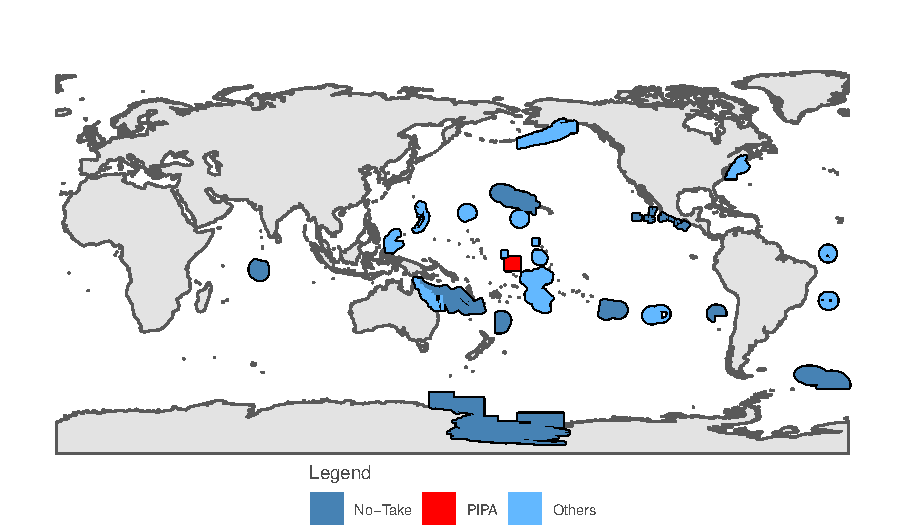
\includegraphics{img/LSMPAs_map.pdf}
\caption{\label{fig:LSMPAs_map}Large Scale Marine Protected Areas. The map shows all areas larger than 30,000 Km\textsuperscript{2}. The Phoenix Islands Protected Area is shown in red.}
\end{figure}

The Phoenix Islands Protected Area (PIPA) in Kiribati is one of the most notable Large-Scale Marine Protected Areas. Implemented on January 1st of 2015, PIPA closed an area of 397,447 km\textsuperscript{2} to fishing and was implemented within an area where approximately 50\% of the world's tuna is caught. Tuna purse seine fisheries in the region are collectively managed under a Vessel-Day Scheme (VDS) by nine countries commonly referred to as the Parties to the Nauru Agreement (PNA). Members include the Federated States of Micronesia, Kiribati, the Marshall Islands, Nauru, Palau, Papua New Guinea, the Solomon Islands, and Tuvalu; Tokelau joined the PNA group in 2012 and started selling access rights in 2013 (Figure \ref{fig:PNA_map}). The Nauru Agreement regulates access of foreign vessels (\emph{i.e.} those from non-PNA countries). Holding 80\% (14.6 million km\textsuperscript{2}) of historical skipjack tuna purse seine grounds within their Exclusive Economic Zones (EEZ), PNA countries have achieved greater bargaining power when providing fishing access to foreign fleets \cite{havice_2010}. The vessel-day price rose from \$5,000 USD in 2012 to at least \$9,000 USD in 2016. The revenue from access fees may represent up to 50\% of government revenue for some of the members.

A spatial closure the size of PIPA is likely to cause changes in spatial distribution and behavior of fishing vessels. For example, the anticipation of LSMPAs may lead to preemptive overfishing, which likely erodes or delays the expected benefits of an intervention \cite{mcdermott_2018,hanich2018unraveling}. Under a VDS, a reduction in total fishing area within one country's EEZ will result in a reduction in license revenues to said country. However, the benefits of the spatial closure are dispersed amongst all other PNA members (through fish movement), who in turn benefit from the conservation efforts of the initial country. While no studies have assessed the implications of PIPA, other PNA members have pledged the implementation of LSMPAs by 2020 (\emph{i.e.} Palau).

We simulate the PNA fishery with the addition of spatial closures to characterize possible outcomes of such interventions. We then empirically evaluate the behavioral responses and spatial redistribution of the industrial tuna purse seine fleet resulting from the implementation of the Phoenix Islands Protected Area, and quantify its economic ramifications and impacts to Kiribati. We use the same data to hypothesize what might be the impacts of the proposed Palau National Marine Sanctuary. These are two of the largest protected areas on the planet and both are controlled by PNA countries, where the largest tuna fisheries occur.

Our empirical portion uses identification of fishing activity via Automatic Identification Systems (AIS) to track 313 tuna purse seine vessels that fished in PNA waters between 2012 and 2018. We continuously observe 92 vessels for the 2012 - 2018 period. Of these, 64 vessels fished within PIPA at least once prior to its implementation, and refer to them as the ``displaced vessels''. The remaining 28 vessels never fished in PIPA waters, and we refer to them as ``non-displaced vessels''. The group with the remaining 221 vessels contains vessels that were not continuously observed before and after the implementation of PIPA, and we refer to these as ``other vessels''.

\begin{figure}[htbp]
\centering
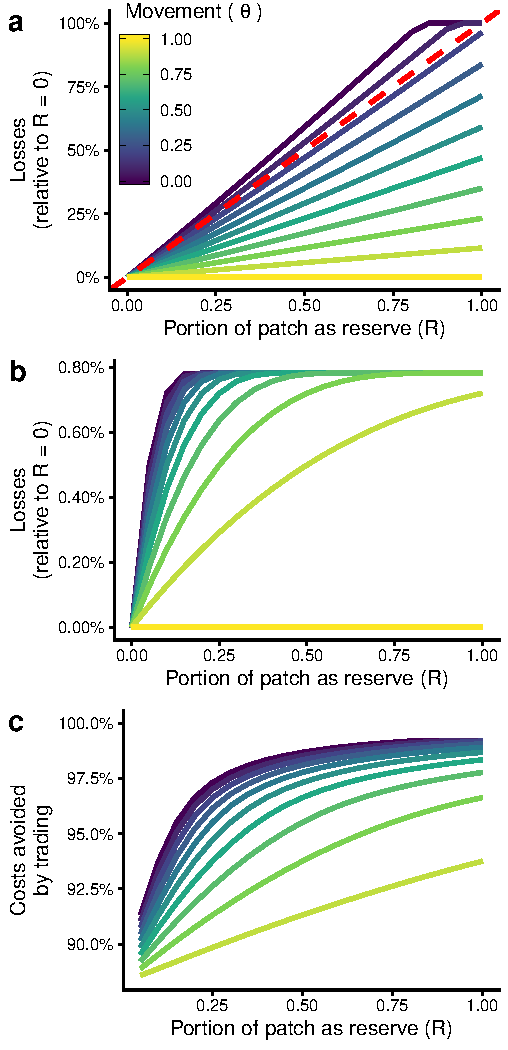
\includegraphics{img/PNA_model.pdf}
\caption{\label{fig:PNA_model}Change in revenue from the PNA model with conservation. Revenue is shown for Kiribati alone (A) and all other PNA countries (B) as a function of increasing proportion of patch as reserve ($R$). Each line (color) represents a value of the movement parameter $\theta$.}
\end{figure}

\section{Results}\label{results}

\subsection{PNA model with conservation}

We simulate the PNA as a ten-patch meta-population system with discrete time, where Patch 1 considers the implementation of a spatial closure. Patches 2-9 are the other PNA countries, and Patch 10 represents the high seas and non-PNA countries. The stock remains within a Patch during the season, but escapement (\emph{i.e.} stock minus catches) is distributed between all countries at the end of each year. A detailed explanation of the model is presented in the Methods section. We find that a spatial closure in Patch 1 always results in a loss or no-change in revenue from vessel-days, even when the stock to moves freely between the protected and non-protected portion of the Patch. The loss in revenue increases with reserve size, but decreases as within-patch movement increases (Fig. \ref{fig:PNA_model}A). For all other PNA countries, however, a spatial closure in Patch 1 results beneficial, especially as within-patch movement decreases and reserve size increase (Fig. \ref{fig:PNA_model}B). The inverse effects of the spatial closure on Kiribati and the other PNA countries are driven by the redistribution of escapement. The stock not fished in the protected portion of Patch 1 eventually redistribute to the other patches, which increases stock size and causes vessel-day prices to increase. This model shows that the costs of conservation are incurred by Patch 1, but the benefits are perceived by the other eight patches. Moreover, the gains in revenue for other PNA countries does not compensate for the total losses to Kiribati, as a great portion of effort is redistributed to the High Seas.

\subsection{Empirical analysis}

Spatial distribution and longitudinal shifts of tuna -particularly skipjack- have been linked to ENSO events \cite{lehodey_1997}. Vessels may then redistribute across PNA countries as they track these stocks \cite{aqorau_2018}. To account for environmentally-driven patterns in vessel location, we incorporate the monthly NINO4 anomaly index in our analyses. The NINO4 index is an area-averaged measure of Sea Surface Temperature from 5S-5N and 160E-150W. The NINO4 anomaly index is the same, with the 1981-2010 mean removed, as made available from the Global Climate Observing System (Fig. \ref{fig:nino_plot}).

\subsubsection{Crowding effect}

We first inspect the crowding effects that may arise due to the net reduction in fishing area. We produced 1-degree rasters of monthly fishing effort for our displaced and non-displaced vessels, and calculated two indices of spatial overlap between them: 1) the number of cells that had fishing activity from both groups for each month and 2) the correlation of presence/absence of fishing activity between both groups over one month. We find that the two fleets significantly interact more with each other after the implementation of PIPA (Table \ref{tab:sp_corr} Fig. \ref{fig:sp_corr}). The number of cells with presence from both fleets and spatial correlation increase by a factor of four and three, respectively. This increase in crowding is likely to increase the encounter rates with other vessels, and reduce the efficiency of fishing operations. This might cause vessels to leave their current fishing grounds and re-optimize their spatial effort, leading to a subsequent decrease as the crowding measures return towards pre-implementation levels. These results are robust to a series of specifications, accounting for the addition of satellites and monthly NINO4 anomaly (Table \ref{tab:sp_corr}). A model fit with NINO4 anomaly as the only explanatory variable explained just 3\% and 7\% of the variation in our crowding measures. Similar results are obtained when repeating the exercise for Kiribati only (Table \ref{tab:KIR_sp_corr}, Fig \ref{fig:KIR_sp_corr})

\begin{figure}[ht]
\centering
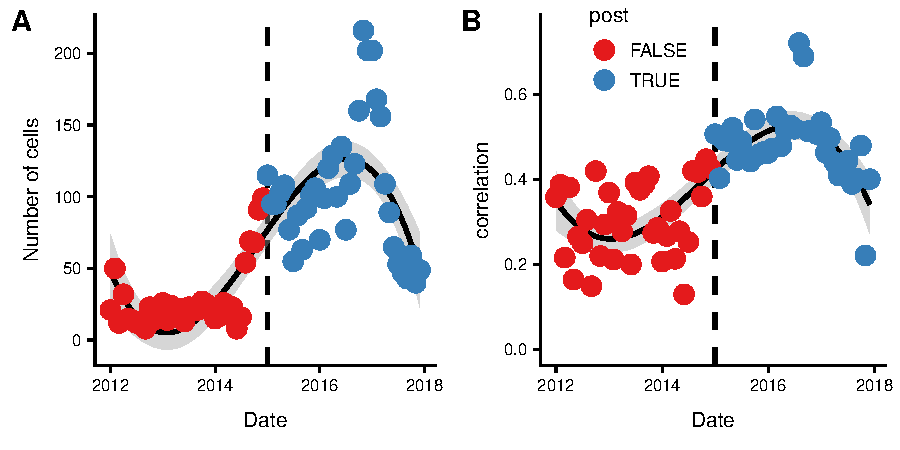
\includegraphics{img/sp_corr.pdf}
\caption{\label{fig:sp_corr}Number of cells that had displaced and non-displaced vessels (A) and spatial correlation in the presence-absence of each group per cell (B). The solid lines represent the 4\textsuperscript{th} degree polynomial fit reported in \ref{tab:sp_corr}. Note that the late 2016 and early 2017 showed negative or neutral NINO4 anomalies, similar to those in the pre-PIPA period.}
\end{figure}

\subsubsection{Behavioral changes}

The behavioral responses that vessels can have to a spatial closure may occur in different ways. For example, displacement to new fishing grounds may represent a cost as fishers search the ocean to identify the most suitable fishing spots. This may result in increased fuel and labor costs. For every vessel in each group, we calculate nine key measures that could capture responses to spatial closures: daily fishing hours, daily non-fishing at-sea hours, the proportion of fishing to non-fishing hours at sea hours, daily distance traveled, daily mean distance from shore of fishing events (km), daily mean distance from port of fishing events (km), as well as monthly hours spent in PNA waters, Kiribati waters, and the High Seas (Fig. \ref{fig:all_panels}). We leverage our Before-After-Control-Impact (BACI) design and implement a log-linear difference-in-differences analysis to evaluate how these measures change for displaced vessels after implementation of PIPA, relative to the trends observed for non-displaced vessels (see the Methods section for our empirical specification). As before, our analyses incorporates monthly NINO4 anomalies to account for possible environmentaly-driven variations.

We find no evidence of displaced vessels fishing for more hours after PIPA implementation, and in fact observe a negative effect (24.3\% decrease; $p < 0.01$; Table \ref{tab:main_DID}) relative to the non-displaced vessels. Likewise, we observe a 3.4\% decrease of fishing hours relative to total at-sea hours ($p < 0.01$; Table \ref{tab:main_DID}). Treated vessels traveled 21\% less distance, with fishing events occurring 28.5\% and 15.7\% closer to shore to port, respectively. These changes in distance from shore and port are likely caused by redistribution, as we observe that displaced vessels fish 58.6\% and 40.3\% less in Kiribati and PNA waters, compared to the trend observed for non-displaced vessels ($p < 0.01$). We do not observe a statistically significant increase in fishing hours on the High Seas.

These patterns suggest that displaced vessels are fishing less overall and this decrease is driven by a decline in fishing within PNA waters. In summary, vessels that used to fish in PIPA are now fishing less in both Kiribati and the PNA region. Vessels that did not use to fish in PIPA are fishing more in Kiribati and PNA waters, with slight increases in the High Seas \ref{fig:fishing_raster_diff}. The results are robust to a set of different specifications, with interaction effects shown in Fig  \ref{fig:other_specifications}. We repeat this analysis for groups where we exclude all Chinese vessels (Table \ref{tab:DID_without_CHN}), all PNA-owned vessels (Table \ref{tab:DID_without_PNA}) and all Taiwanese and USA vessels (Table \ref{tab:DID_without_USA_TWN}) and find qualitatively the same reposnses.

\subsubsection{Economic impacts}

The crowding effect combined with the reduction in hours spent in Kiribati and PNA waters overall suggests that displaced vessels have redistributed elsewhere, meaning that they buy less vessel-days from PNA countries. To quantify the potential impacts of this leakage, we estimate the total annual vessel-days received by Kiribati and all PNA countries by each group of vessels (Fig. \ref{fig:all_PS_VDS_year}), and convert these to license revenues using a conservative vessel-day price of \$9,000 USD\footnote{The Pacific Islands Forum Fisheries Agency \emph{Tuna Development Indicators 2016} report states that ``Days are currently [2016] selling in a range between \$9,000 and \$13,000 USD.''}. We look at all 313 vessels to obtain a more accurate representation of total revenues, but continue to group vessels as displaced (n = 64), non-displaced (n = 28), and other vessels (n = 221).

We find that between 2015 and 2016, displaced vessels spent 3,916 and 2,249 less vessel-days in Kiribati and PNA waters, respectively (Figs. \ref{fig:all_PS_VDS_year} and \ref{fig:included_PS_VDS_year_DiD}). Over the same period, non-displaced and other vessels spent 1,278 less days in Kiribati, but spent 9,853 more days in PNA waters overall. These changes result in a net loss of 5,195 vessel-days for Kiribati, and a net gain of 7,600 vessel-days at the PNA-level (\emph{i.e.} the other 8 countries). The net reduction of vessel-days in Kiribati represents a loss of \$46.7 million USD in vessel-day licenses, while the net gain at the PNA-level results in an increase of \$68 million USD.

Moreover, annual vessel-days in Kiribati continued to decrease to just 7,479 in 2018 (Fig. \ref{fig:all_PS_VDS_KIR_year}). This trend is mainly caused by displaced vessels allocating less time to Kiribati (Figs \ref{fig:all_PS_VDS_KIR_year} and \ref{fig:hist_kir_fishing}). Looking at the total annual vessel-days allocated by all vessels to all countries, we see that the largest reductions occur for Kiribati, while Papua New Guinea exhibits a proportional increase (Fig. \ref{fig:all_PS_VDS_cty_year}).

\begin{figure}[ht]
\centering
	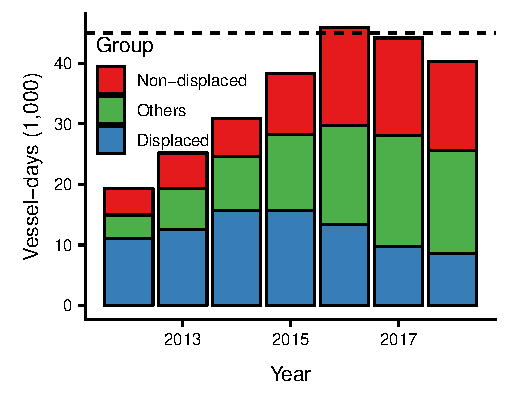
\includegraphics{img/all_PS_VDS_year.pdf}
	\caption{\label{fig:all_PS_VDS_year}Observed vessel-days for all PNA countries by displaced, non-displaced, and other vessels.}
\end{figure}

\begin{figure}[ht]
\centering
	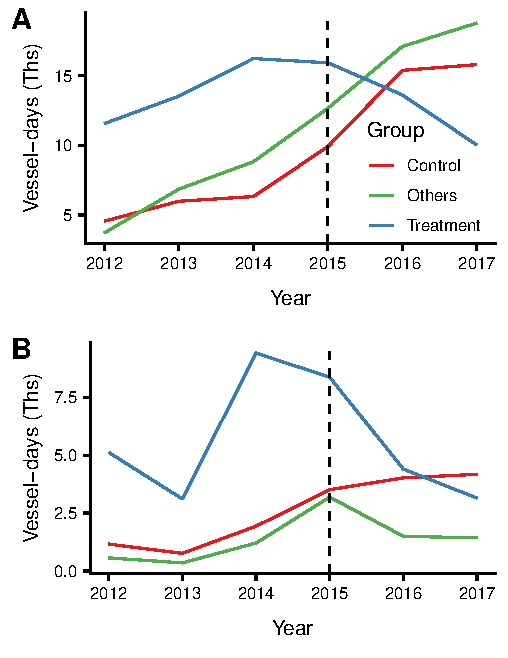
\includegraphics{img/included_PS_VDS_year_DiD.pdf}
	\caption{\label{fig:included_PS_VDS_year_DiD}Vessel days spent inside A) PNA waters and B) Kiribati waters by vessel group. The large increase for Kiribati in 2014 is likely explained by the blue paradox \cite{mcdermott_2018}}
\end{figure}

We complement our analysis of change in observed vessel-days by looking at country-level data. Specifically, we use data compiled by the Pacific Islands Forum Fisheries Agency (FFA\footnote{https://www.ffa.int/node/2050}) where annual revenues from license fees are reported for each country (2008 - 2016; Fig. \ref{fig:revenues}A). We find that Kiribati's revenue went from \$148.8 million USD in 2015 to \$118.3 million USD in 2016, representing a decrease of \$30.5 million USD. However, total PNA revenues showed a net increase of \$28 million USD (Fig. \ref{fig:total_PNA_revenues}). The largest decrease was observed for Kiribati, while the largest increase was observed for Papua New Guinea.

\begin{figure}[ht]
\centering
	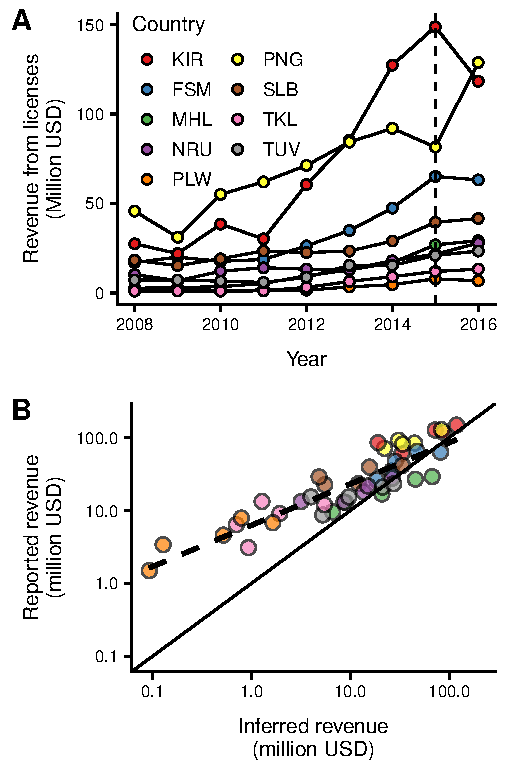
\includegraphics{img/revenues.pdf}
	\caption{\label{fig:revenues}
		License revenue for PNA countries. A) Annual revenue from fishing license fees by country and year (2008 - 2016) B) $log_{10}$-transformed FFA-reported revenues vs. the revenues inferred from vessel activity observations (2012 - 2016). The dashed line represents line of best fit, solid line represents 1:1 line. The same graph using absolute values is shown in \ref{fig:revenue_FFA_GFW_linear}.}
\end{figure}

Catch for each country's EEZ for the 1997 - 2016 period were also obtained from the FFA (Fig. \ref{fig:catches}). Catches in Kiribati waters decreased from 24,051 to 12,894 tonnes between 2015 and 2016 (46.3\% decrease). Similar decreases were observed for The Federated States of Micronesia (60.9\%), Papua New Guinea (43.4\%) and the Solomon Islands (58.5\%). In contrast, Tokelau (due south of PIPA) showed a 22.3\% increase in catch over the same period.

\subsection{Potential Revenue Loss for Palau}

On October 28, 2015, the President of Palau signed into law the Palau National Marine Sanctuary (PNMS) Act. Starting in December 2020, this Act will close 500,000 km\textsuperscript{2} to commercial fishing activities, creating the 14th largest protected area in the world. The sanctuary will fully protect about 80 percent of Palau’s EEZ. Table \ref{tab:revenue_loss} presents estimates of the potential revenue losses following full enactment of the PNMS under four different scenarios. In Scenario 1, Palau is able to keep its current allotment of purse seine vessel days (700) and is able to sell them for a similar price to what it is currently selling them to the United States for under the South Pacific Tuna Treaty also known as the Multilateral Treaty on Fisheries (\$12,500/day). In Scenario 2, Palau is able to keep its current allotment of purse seine vessel days (700) to transfer to other PNA countries at the current benchmark price (\$8,000/day). Scenario 2 is likely if Palau retains its current allocation, but the US no longer purchases days.  It should be noted that if allocation continues to be calculated based on effort and biomass, and if Palau continues to be allocated vessel days, its allocation will decrease as effort in its EEZ reaches zero. In Scenarios 3 and 4, Palau loses all of its PS vessel days, at \$8,000/day and \$12,500/day, respectively. In all scenarios, all longline vessel day and export tax revenues are lost, since longline vessel days are currently not tradable and Palau is planning on banning the export of fish. The longline vessel day loss is calculated using an average value of \$200 for 10,500 days. The export tax loss is calculated given the average tax revenue from 2012-2014 (\$482,236  from \cite{Gillett2016}). 

\begin{table}[htbp] \centering 
	\caption{Estimated revenue losses under different scenarios of PNMS (in USD)} 
	\label{tab:revenue_loss} 

\begin{tabular}{l*{5}c}

\hline
\hline
Scenario	&	PS VDS	&	LL VDS	&	Export tax	&	Total revenue loss	\\
\hline
	1	&	0	&	-2,100,000	&	-482,236	&	-2,582,236	\\
	2	&	-3,150,000	&	-2,100,000	&	-482,236	&	-5,732,236	\\
	3	&	-5,600,000	&	-2,100,000	&	-482,236	&	-8,182,236	\\
	4	&	-8,750,000	&	-2,100,000	&	-482,236	&	-11,332,236 	\\
	
	\hline 
	\hline
	
\end{tabular} 




\end{table}

\section{Discussion}

Our findings provide insights into the effect that LSMPAs can have on redistribution of fishing effort and change in behavior. Our simulation predicts losses in revenue to countries that implement a spatial closure, increases in revenue to other countries, and an increased fishing of the high seas. Using vessel track data, we observe a crowding effect after the implementation of the protected area, as displaced vessels redistribute spatially. We see that vessels that fished inside PIPA before the implementation redistributes to other areas within Kiribati, but also other PNA countries and the high seas. Our analysis shows that the implementation of PIPA had little effect on the \emph{total} fishing effort exerted by purse seiners. Surprisingly, there is no drop off in fishing effort in Kiribati in 2015 but a noticeable drop from 2016 onwards. Our analysis suggests that the displacement of vessels results in losses to Kiribati, and that similar outcomes would be expected for Palau's Marine Sanctuary with losses in profits of up to \$11 million USD. Here, we discuss the implications of our findings and possible shortcomings in our analysis.

Previous studies on protected areas around Pacific islands suggest that vessels move to distant places, which might be translated as increased costs \citep{stevenson_2013}. Others have used similar satellite-tracking systems to show that fishing effort accumulates near the edges of spatial closures, yielding greater catches over time \citep{murawski_2005}. But these vessel tracks do not cover the pre-reserve period, making it difficult to identify the contribution of spatial closures to the observed spatial distribution of fishing vessels. Recent work by \cite{elahi_2018} identified that total fishing effort in a focal region where a short-term MPA was implemented showed little change, likely indicating that fishers redistributed fishing effort to compensate for the reduction in available space. Our data, which is assembled in a similar way, allows us to make similar inferences about the unobserved change in aggregate fishing effort and its spatial redistribution.

Our analysis of vessel-days from vessel tracks and loss of profits to Kiribati suggests losses of \$46.7 million USD, while revenue data show a decrease in only \$30 million USD. Here, we provide some plausible explanations for these discrepancies. First, it is possible that as waters in Kiribati became more crowded, the price of vessel-days decreased significantly bellow the \$9,000 USD estimate that we use. This woudl imply that vessel-day prices fell to \$5,800 in Kiribati. This is a number similar to what our simulation estimates provide for a closure similar to PIPA (\emph{i.e.} $R = 0.11$), which range from \$5,250 to \$6,134, depending on the movement of fish. Another possible explanation is that the dataset used incorrectly labeled vessels as purse seiners. However, the scoring algorithm has a high accuracy, and this accuracy increases with the number of observations for a vessel. Moreover, on any given year, 90\% of total fishing activity can be explained by 68\% to 75\% of the vessels (Fig \ref{fig:nvessels_to_90}). Therefore, if there are any mislabeled vessels in our data, these would contribute little to the large trends that we observe. Another alternative is that vessels fishing within PNA waters can report their activity as transiting to port or solving mechanical issues; this time does not count towards a vessel's usage of days (forgot the reference). Finally, Kiribati's vessel-day allocation is in the order of 7,000 vessel-days (need reference). However, we observe that on any given year, Kiribati received between 3,000 and 14,900 vessel-days (Fig \ref{fig:all_PS_VDS_KIR_year}), implying that a portion of these were purchased or transfered from other PNA countries. These explanations are not mutually exclusive, and a combination of them could certainly explain the discrepancy. While the magnitude is not the same, the trends and patterns through time are certainly similar, and all indicate a reduction of usage of Kiribati's waters.

ENSO events are known to drive the behavior of fishing vessels, especially in PNA waters, which may drive reallocation of fishing effort \cite{lehodey_1997,kroodsma_2018,aqorau_2018}. We do our best control for these environmental changes by incorporating the NINO4 anomaly index in our analyses, and by tracking non-displaced vessels as a group that is equally affected by the environmental variation. For example, we observe that both displaced and non-displaced vessels shifted their effort to the Western margin of the PNA region, namely Kiribati's Gilbert Islands and Tuvalu. However, displaced vessels redistribute a greater proportion of fishing effort to these areas, as well as the High Seas (Fig \ref{fig:fishing_raster_diff}). Our analysis shows that sea surface temperature variation does have an effect on our crowding and behaviroal methods, but that by itself does not explain the observed patterns. While environmental variation certainly influences behavior, policy and management interventions such as moratorium and spatial closures can have an equally big effects \cite{kroodsma_2018}.

A major shortcoming of our analysis is that we do not observe catch or revenue at the vessel level, which ultimately guide the decision-making process of profit-maximizing agents. Therefore, it is difficult to know whether the small change in fishing hours and redistribution represents a positive or negative impact. Likewise, the available data from the FFA does not cover the 2017 and 2018 period, and we do not observe vessel-day transactions or prices. Furthernore, our estimates of revenue loss for PIPA do not account for the allocation calculated each year. Each party’s allowable effort is calculated based on historic effort and biomass within each party’s EEZ. Sixty percent of the PAE is calculated based on EEZ effort over the last seven years and 40\% is calculated based on the 10-year average of each country’s share of estimated skipjack and yellowfin biomass within its EEZ.\footnote{This is explained in more detail in Article 12.5 of the 2012 Amendment to the Palau Agreement and in \cite{Hagrannsoknir2014}}.

Our work suggests that the implementation of a Large-Scale Marine Protected Areaa had little impact on total fishing effort, but that it may result in revenue losses. The closure caused a crowding effect, which causes some vessels to redistribute to areas close by. The Parties to the Nauru Agreement have shown that multinational cooperation in management of transboundary resources can have management and economic benefits \cite{lehodey_1997,aqorau_2018}. Overlaying conservation interventions over existing management schemes must be accompained by similar dialogues and international cooperation, so that the benefits of conservation are captured by those incurring the costs. Furthermore implementation of Large-Scale Marine Protected Areas must be accompanied by traditional fisheries management to maximize effectivenes, consider the opportunity costs of such closures \cite{smith_2010}, and identify sustainable financing mechanisms\cite{mallin_2019} that would compensate losses and incentivize marine conservation in the long term.

\begin{scriptsize}

\section{Methods}

\subsection{PNA Model with Conservation}

We model the PNA as a ten-patch discrete-time meta-population system, where Patch 1 is considering a spatial closure. Patches 2-9 are the other PNA countries, and Patch 10 represents the high seas and non-PNA countries. The stock of fish in each country is relatively stationary within a single fishing season, but redistributes across all patches annually. The price of fish is $p$, and catchability is given by $q$.

In the absence of a reserve, the revenue for vessels in patch $i$ is given by $pqE_iX_i$, where $E_i$ and $X_i$ are effort (vessel-days) and stock size in patch $i$ at the beginning of a period. The cost of fishing in patch $i$ is given by $cE_i^\beta$, where $\beta = 1.3$ matches commonly-used cost functions. Patch 1 considers a spatial closure by implementing a reserve as a fraction $R$ of the total patch ($R \in[0,1]$). Fish move within a patch based on $\theta$, where $\theta = 0$ implies to movement within the patch, and $\theta = 1$ implies that fish within the patch are well mixed over during the fishing season. In this patch, revenues are given by $pqE_1X1(\theta + (1 - \theta)(1 - R))$. The parameterization of movement and reserve size imply that profit from fishing Patch 1 is given by:

\begin{figure}[H]	
	\begin{align}
	\Pi_1(E_1,X_1,R) = pqE_1X_1(\theta + (1 - \theta)(1 - R))-cE_1^\beta
	\end{align}
\end{figure}

And profits from fishing in Patch $j = \{2, 3, ..., 10\}$ are:

\begin{figure}[H]	
	\begin{align}
	\Pi_j(E_j,X_j) = pqE_jX_j-cE_1^\beta
	\end{align}
\end{figure}

The above equations imply that the marginal profit from the last unit of effort in a patch are given by:

\begin{figure}[H]	
	\begin{align}
	\pi_1(E_1) = pqX_1(\theta + (1 - \theta)(1 - R)) - \beta cE_1^{\beta-1}
	\label{eqn:marginal_profit_1}
	\\
	\pi_j(E_j) = pqX_j - \beta cE_j^{\beta-1}
	\label{eqn:marginal_profit_j}
	\end{align}
\end{figure}

However, Patch 10 represents the high seas under open access dynamics. Therefore, we assume that effort continues to enter Patch 10 until the profit from the last unit of effort is exactly zero, indicating that $E_{10}$ is the value for which $\pi E_{10} = 0$. Setting Equation \ref{eqn:marginal_profit_j} equal to zero and solving for $E_j$ gives:

\begin{figure}[H]	
	\begin{align}
	E_{10} = \left(\frac{pqX_{10}}{\beta c}\right)^{\frac{1}{(\beta - 1)}}
	\label{eqn:effort_hs}
	\end{align}
\end{figure}

The patch-level harvest is then determined by effort and stock size:

\begin{figure}[H]	
	\begin{align}
	H_1 = qE_1X_1 (\theta + (1 - \theta)(1 - R))
	\label{eqn:harvest_1}
	\\
	H_j = qE_jX_j
	\label{eqn:harvest_j}
	\end{align}
\end{figure}

Therefore, escapement in patch $i$ is the difference between initial stock size and harvests as $e_{it} = X{it} - H_{it}$. At the entire stock then grows according to:

\begin{figure}[H]	
	\begin{align}
	X_{t+1} = e_t + \frac{(\phi + 1)}{\phi}ge_t\left(1 - \left(\frac{e_t}{K}\right) ^{\phi}\right)
	\label{eqn:grow}
	\end{align}
\end{figure}

After the stock grows, a constant and patch-specific fraction $f_i$ of the total stock redistributes to patch $i$, so:

\begin{figure}[H]	
	\begin{align}
	X_{it+1} = f_iX_{t+1}
	\label{eqn:disperse}
	\end{align}
\end{figure}

The vessel-day price that a country charges is given by $\pi_i$ from Equations \ref{eqn:marginal_profit_1} and \ref{eqn:marginal_profit_j}. Therefore, patch-level license revenues are given by:

\begin{figure}[H]	
	\begin{align}
	\omega = \pi_iE_i
	\label{eqn:license_revenue}
	\end{align}
\end{figure}

Equations \ref{eqn:harvest_1} shows that low values of $\theta$ and $R > 0$ would increase escapement, which would lead to an increase in stock size (Equation \ref{eqn:grow}). This would cause for the stock in the high seas ($X_{10}$) to increase through the redistribution (Equation \ref{eqn:disperse}), leading to an increased effort being allocated to the high seas (Equation \ref{eqn:effort_hs}).

\subsection{Data}

Automatic Identification Systems (AIS) are on-board devices that provide at-sea safety and prevent ship collisions by broadcasting vessel position, course, and activity to surrounding vessels. These broadcast messages can be received by satellites and land-based antennas. GFW then uses machine learning algorithms (convolutional neural networks) on the broadcast messages to infer type and location of fishing events \citep{kroodsma_2018}.

The amount of data gathered by GFW is dependent on the number of antennas and satellites that can receive signals. The total satellite count increased from 3 to 6 on June 1\textsuperscript{st} 2014 , and then from 6 to 10 on January 1\textsuperscript{st} 2016. This causes an increase in the number of \emph{received} AIS messages (\emph{i.e.} points), and therefore an apparent increase in the number of vessels. The addition of new satellites affects all vessels in the same way.

Our treatment group contains all purse seiners (n = 64) that fished within PIPA at least once before the announcement, and that continued to fish elsewhere after the January 2015 implementation. Vessels in the non-displaced group meet the following two conditions: i) never fished within PIPA waters from 2012-2015, and ii) vessels have fished in surrounding areas (\emph{i.e.} PNA-countries' EEZ) before and after PIPA closure (n = 28). Together, these vessels represent more than 20 million georeferenced positions for which we know activity (fishing or not fishing). We include three additional control groups as a robustness check. The first group excludes all Chinese vessels, the second group excludes all PNA vessels, and the third group excludes US and Taiwanese vessels. Our main definition of displaced and non-displaced groups leaves us with 64 displaced and 28 non-displaced vessels, which have just over 36 million observations.

\subsection{Analysis}

\subsubsection{Crowding effect}

\begin{figure}[H]
	\begin{align}
	y_t = \alpha + \beta_1 M_t + \beta_2 M_t^2 + \beta_3 M_t^3 + \beta_4 M_t ^4 + \sigma_s + \mu N_t + \epsilon_t
	\label{eqn:sp_corr}
	\end{align}
\end{figure}

We test for a crowding effect using the specification in Equation [\ref{eqn:sp_corr}]. We have two different outcome variables:
1) the number of cells that had fishing activity from displaced and non-displaced vessels for each month and 2) the correlation of presence/absence of fishing events between both groups over one month.We allow for the possibility of three inflection points: 1) initial crowding due to MPA implementation, 2) When the crowding has reached its peak and star  ts to decrease, and 3) when this decrease potentially levels off. For this reason, we fit a 4th degree polynomial to our monthly indices. We do so by centering our time series of crowding indices on the day of implementation. Our explanatory variable is therefore the number of months ($M$) before or after the implementation. For example, since PIPA was implemented in January 1st of 2015, December of 2014 has a value of -1 and Feb of 2015 would receive a value of 1. Note that we restrict the sample to our displaced and non-displaced vessels (vessels that show up in the dataset before PIPA implementation) to try to minimize bias from more and more vessels using AIS over time. We also include controls ($\sigma_s$) that captures the effect of additional satellites receiving AIS signals, which incorporated in April 1st, 2014 and December 31st, 2015. The$mu$ coefficient captures the effect of the NINO4 anomaly.

\subsubsection{Behavioral changes}

We attempt to identify the response of vessels to the PIPA closure. We use daily fishing and non-fishing hours, daily proportion of fishing vs. non-fishing hours, daily distance traveled (km), distance from shore (km) and distance from home port (km) for fishing and non-fishing events, and proportion of total fishing hours allocated to Kiribati waters and PNA waters as our main outcomes of interest. We compare these outcomes before and after the implementation of PIPA using a Difference-in-Differences approach. 

Our main specification is the following:

\begin{figure}[H]
\begin{align}
log(y)_{i,t} = \alpha + \beta_1 P_t + \beta_2 D_i + \beta_3 P_t \times D_i + \phi_t + \gamma_i + \epsilon_{i,t}
\label{eqn:did}
\end{align}
\end{figure}

\noindent where $log(y_{i,t})$ is the hyperbolic-sine transformation\footnote{$ln\left(y + \sqrt{1 + y^2}\right)\rightarrow ln(2y)$ the transformation was not applied to the proportion of fishing to non-fishing hours.} of the outcome of interest for vessel $i$ on period $t$. A dummy variable $Post_t$ takes the value of 0 for all dates prior to PIPA implementation and a value of 1 for all dates following PIPA implementation. $Treat_i$ is a dummy variable indicating whether a vessel belongs to the displaced ($D_i = 1$) or non-displaced ($D_i = 0$) group. $\alpha$ is the standard intercept term, $\beta_1$ captures the temporal trend, $\beta_2$ captures the initial difference between displaced and non-displaced groups, and $\beta_3$ is our parameter of interest: the Difference-in-Differences estimate capturing the treatment effect. Finally, $\phi_t$ and $\gamma_i$ represent month and flag dummies that account for seasonality or country-level management interventions. 

\begin{comment}
We test for other more complex specifications that interact a quarterly dummy or year-month dummies with the treatment group and find qualitatively the same results\footnote{I actually need more time to run these, but I don't think they'll change}.
\end{comment}

All regression coefficients were estimated via ordinary least squares, and heteroskedasticity-robust standard errors were calculated. All analyses were performed in R version 3.5.1 \citep{rcore_2018}. Raw data and code used in this work are available on \href{https://github.com/jcvdav/MPA_displacement}{github}.

\subsubsection{Revenues}

We obtained information on revenues from the Pacific Islands Forum Fisheries Agency \emph{Tuna Development Indicators 2016} report. For countries in the PNA, these revenues show a combination of vessel-day license fees as well as joint-venture operations.

\end{scriptsize}

\section{References}

\bibliography{references}

%%%%%%%%%%%%%%%%%%%%%%%%%%%%%%%%%%%%%%%%%
%%%%%%%%%%%%%		 					 %%%%%%%%%%%%%
%%%%%%%%%%%%%		 BEGIN APPENDIX		 %%%%%%%%%%%%%
%%%%%%%%%%%%%		 					 %%%%%%%%%%%%%
%%%%%%%%%%%%%%%%%%%%%%%%%%%%%%%%%%%%%%%%%

\clearpage

\onecolumn

\FloatBarrier

\newcommand{\beginsupplement}{\setcounter{table}{0}  \renewcommand{\thetable}{S\arabic{table}} \setcounter{figure}{0} \renewcommand{\thefigure}{S\arabic{figure}}}

\setcounter{table}{0}  \renewcommand{\thetable}{S\arabic{table}} \setcounter{figure}{0} \renewcommand{\thefigure}{S\arabic{figure}}

\section{Supplementary tables and figures}

\begin{figure}[H]
\centering
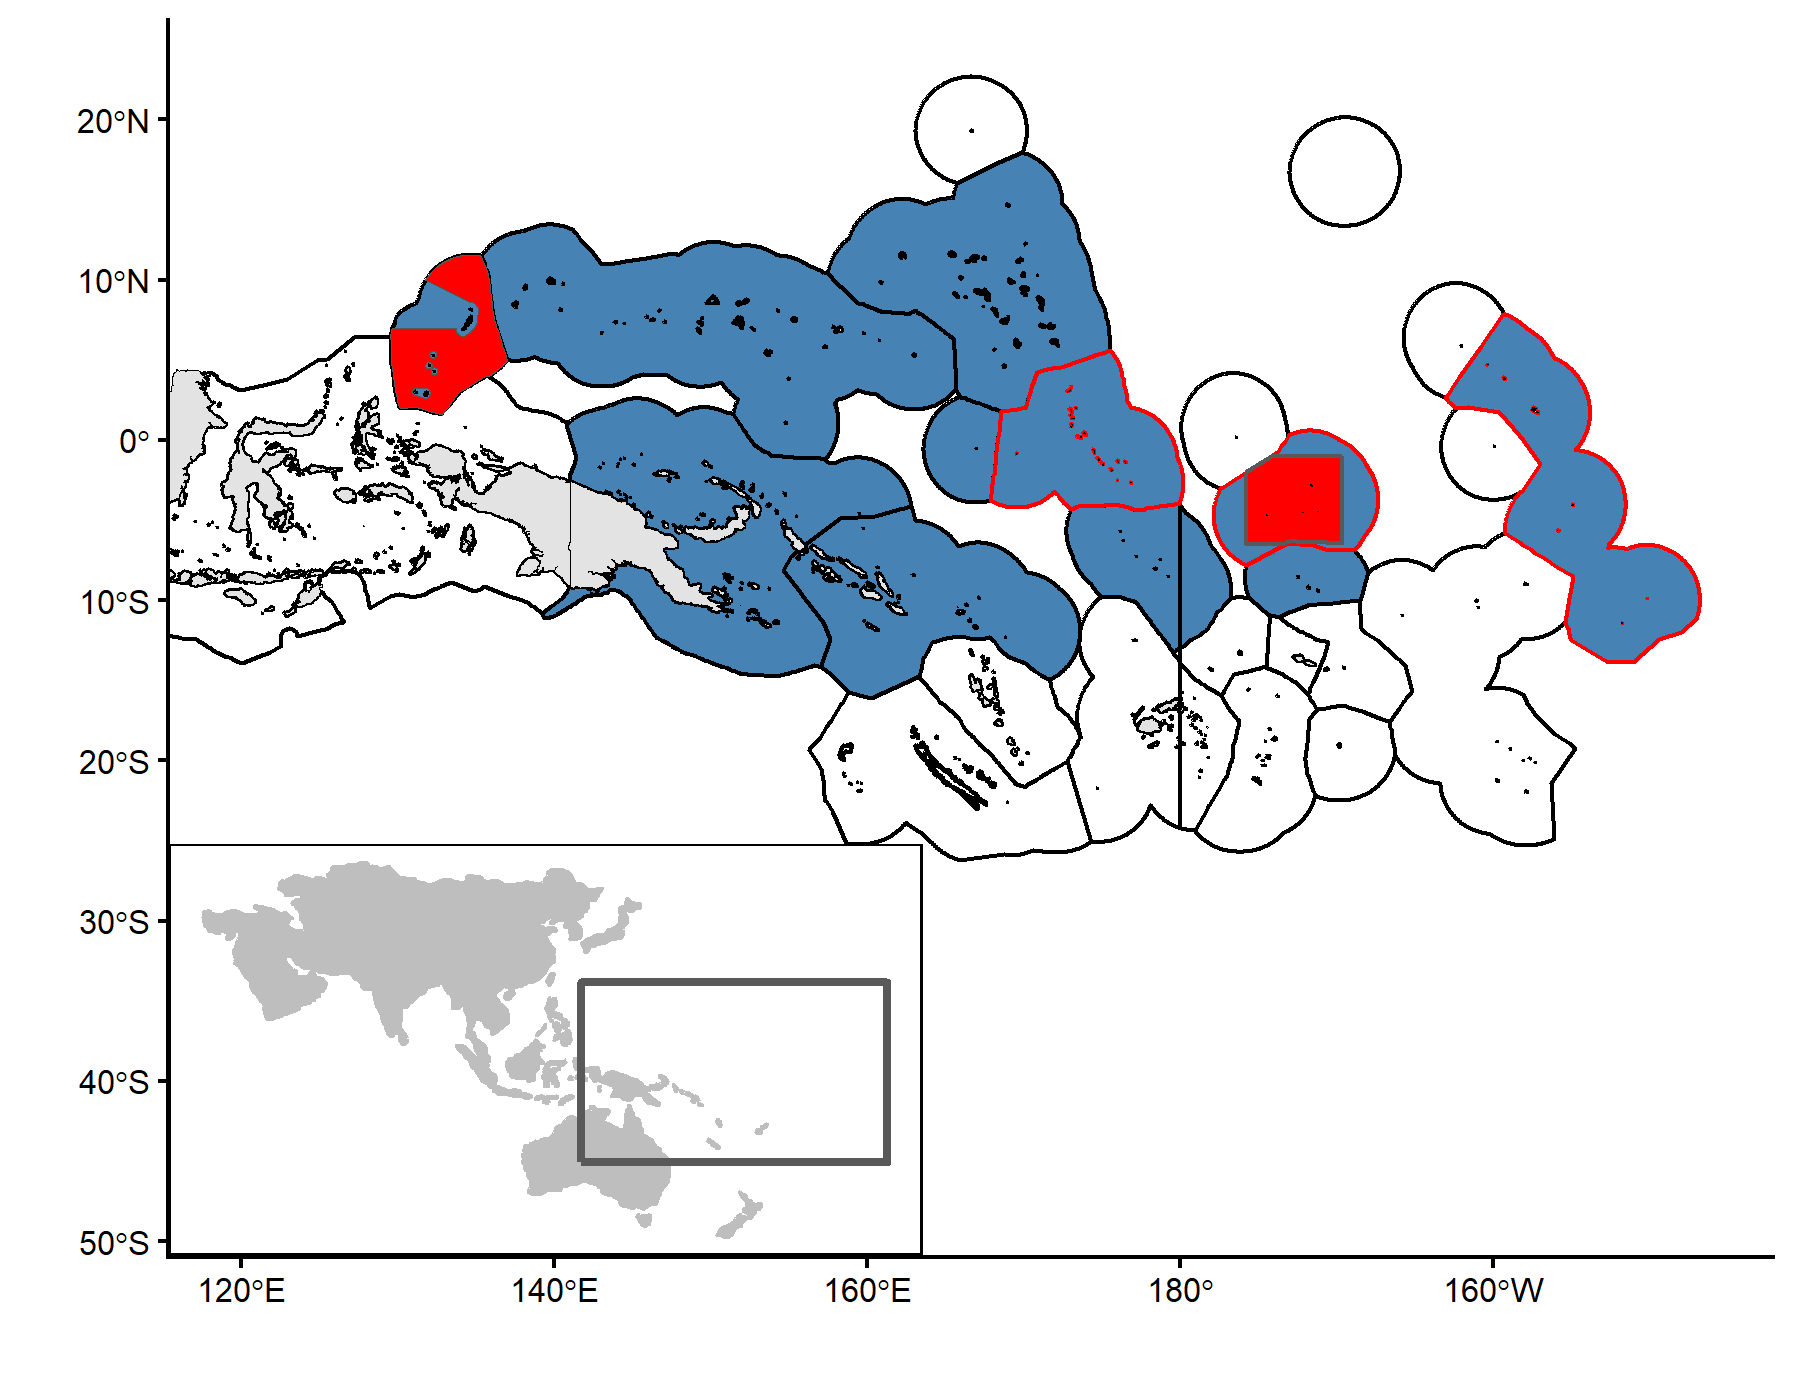
\includegraphics{img/PNA_map.png}
\caption{\label{fig:PNA_map}Map of the Exclusive Economic Zones (EEZs) of the region of interest. Countries that belong to the PNA are shown in blue, while empty polygons indicates all others. A red line indicates the Kiribati EEZ, and a solid red polygon delineates PIPA. Land masses are shown in gray. Labels indicate ISO3 country codes (PLW: Palau, PNG: Papua New Guinea, FSM: Federal States of Micronesia, SLB: Solomon Islands, NRU: Nauru, MHL: Marshal Islands, KIR: Kiribati, TUV: Tuvalu, TKL: Tokelau).}
\end{figure}

\begin{figure}[H]
\centering
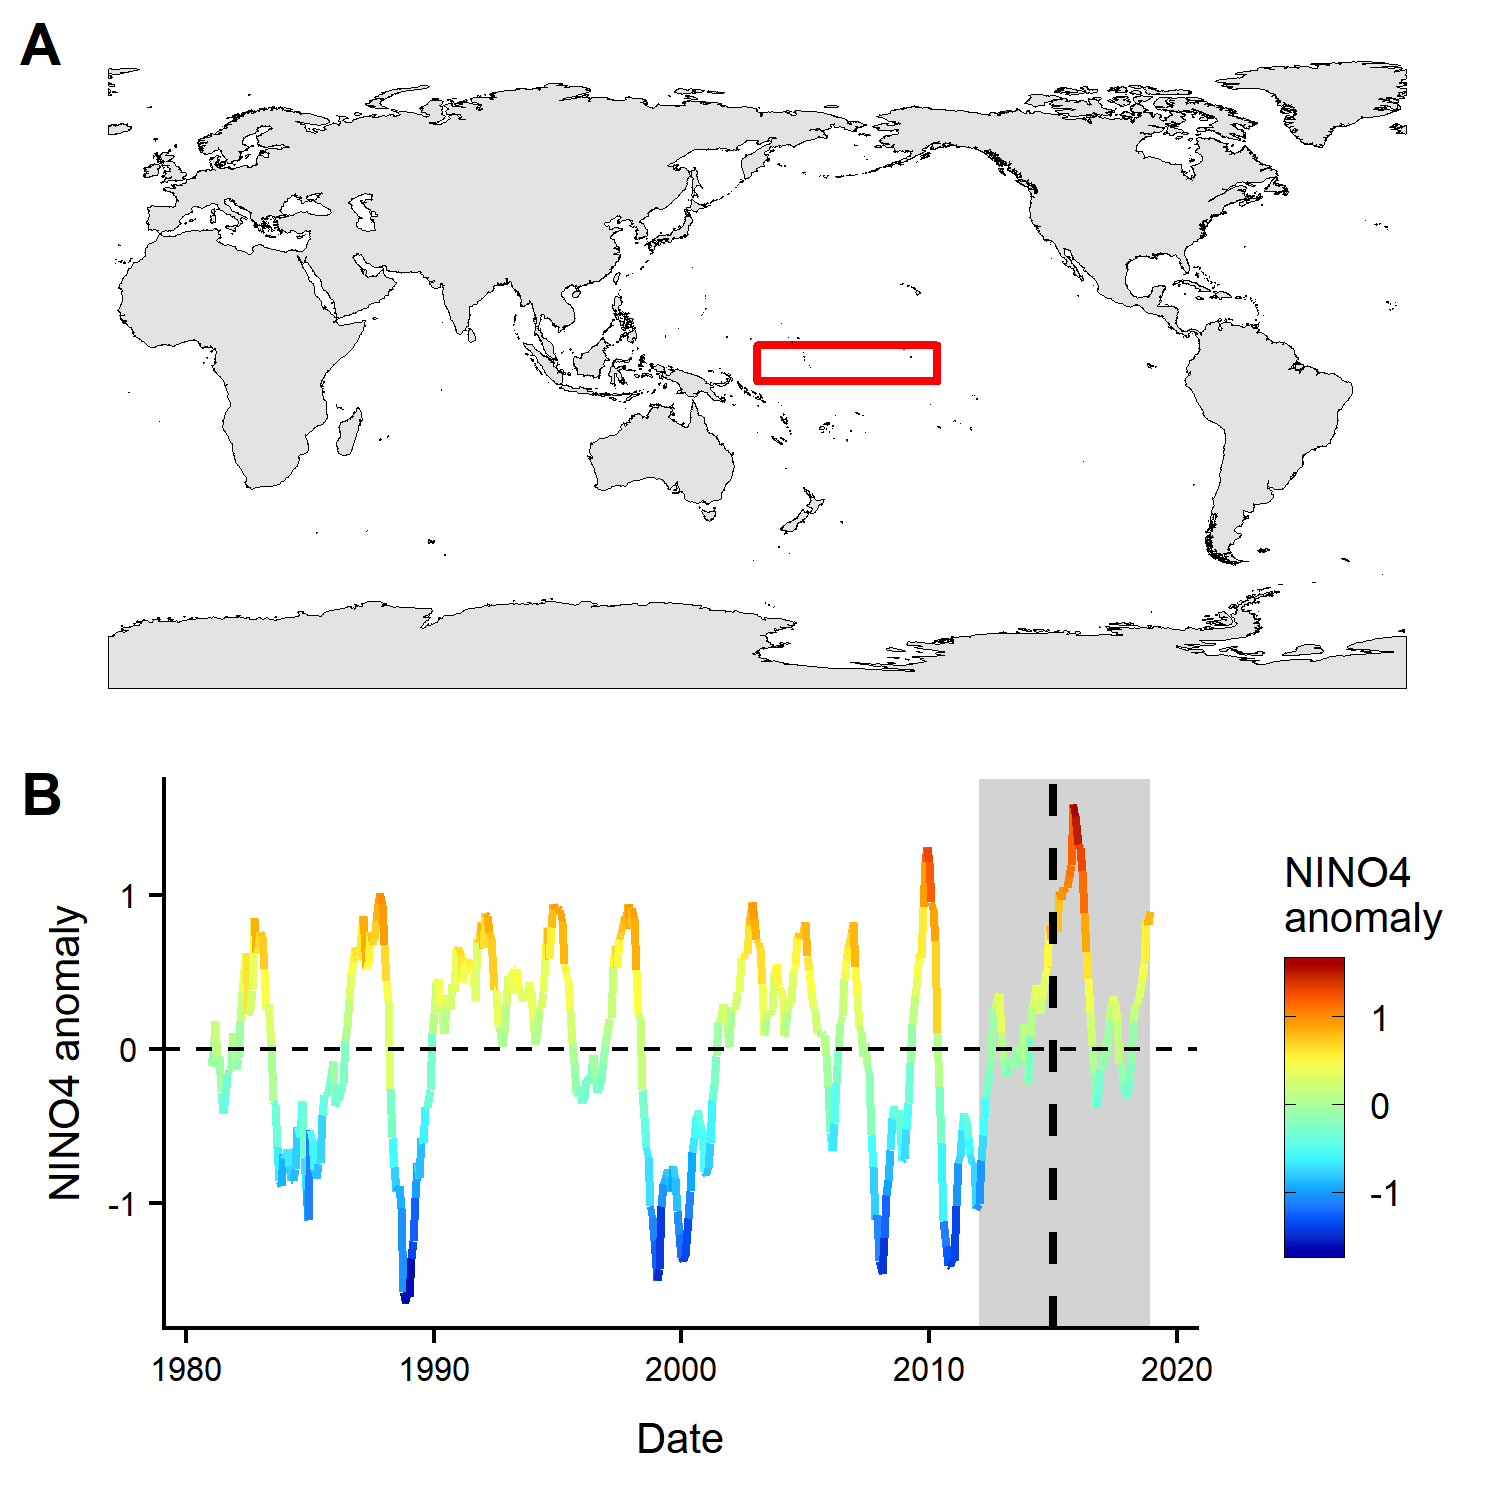
\includegraphics{img/nino_plot.png}
\caption{\label{fig:nino_plot}NINO4 anomaly index. A) Map of the NINO4 region (5S-5N and 160E-150W). B) Timeseries of NINO4 anomaly from January, 1980 to December, 2018.}
\end{figure}

\clearpage


\begin{table}[!htbp] \centering 
  \caption{\label{tab:sp_corr}Coefficient estimates for a third-polinomial fit to the measures of crowding. The first column shows coefficients for the number of cells with treated and control vessels during the same month. The second column shows coefficients for the spatial correlation for presence / absence of treated and control vessels. The explanatory variable is the number of months before implementation of PIPA. Numbers in parentheses are heteroskedastic-robust standard errors.} 
  \label{} 
\footnotesize 
\begin{tabular}{@{\extracolsep{1pt}}lcccccccc} 
\\[-1.8ex]\hline 
\hline \\[-1.8ex] 
\\[-1.8ex] & (1) & (2) & (3) & (4) & (5) & (6) & (7) & (8)\\ 
\hline \\[-1.8ex] 
 Constant & 78.040$^{***}$ & 84.639$^{***}$ & 60.962$^{***}$ & 66.725$^{***}$ & 0.412$^{***}$ & 0.417$^{***}$ & 0.370$^{***}$ & 0.377$^{***}$ \\ 
  & (5.438) & (8.990) & (15.598) & (15.988) & (0.014) & (0.032) & (0.062) & (0.066) \\ 
  & & & & & & & & \\ 
 M & 3.943$^{***}$ & 4.065$^{***}$ & 3.066$^{***}$ & 3.139$^{***}$ & 0.010$^{***}$ & 0.010$^{***}$ & 0.009$^{**}$ & 0.009$^{**}$ \\ 
  & (0.302) & (0.348) & (0.966) & (1.040) & (0.001) & (0.001) & (0.003) & (0.004) \\ 
  & & & & & & & & \\ 
 M $^2$ & $-$0.005 & $-$0.021 & 0.008 & $-$0.008 & $-$0.0001$^{***}$ & $-$0.0001 & $-$0.0001 & $-$0.0001 \\ 
  & (0.019) & (0.026) & (0.027) & (0.030) & (0.00004) & (0.0001) & (0.0001) & (0.0001) \\ 
  & & & & & & & & \\ 
 M $^3$ & $-$0.002$^{***}$ & $-$0.002$^{***}$ & $-$0.002$^{***}$ & $-$0.002$^{***}$ & $-$0.00001$^{***}$ & $-$0.00001$^{***}$ & $-$0.00001$^{***}$ & $-$0.00001$^{***}$ \\ 
  & (0.0003) & (0.0003) & (0.001) & (0.001) & (0.00000) & (0.00000) & (0.00000) & (0.00000) \\ 
  & & & & & & & & \\ 
 M $^4$ & 0.00001 & 0.00002 & 0.00000 & 0.00001 & 0.00000$^{***}$ & 0.00000$^{**}$ & 0.00000 & 0.00000 \\ 
  & (0.00001) & (0.00002) & (0.00002) & (0.00002) & (0.00000) & (0.00000) & (0.00000) & (0.00000) \\ 
  & & & & & & & & \\ 
 NINO4 &  & $-$8.095 &  & $-$10.395 &  & $-$0.006 &  & $-$0.014 \\ 
  &  & (8.287) &  & (9.481) &  & (0.029) &  & (0.031) \\ 
  & & & & & & & & \\ 
 $\sigma_1$ &  &  & 21.318 & 25.102 &  &  & 0.057 & 0.062 \\ 
  &  &  & (19.493) & (22.486) &  &  & (0.076) & (0.080) \\ 
  & & & & & & & & \\ 
 $\sigma_2$ &  &  & 5.299 & 3.194 &  &  & $-$0.015 & $-$0.018 \\ 
  &  &  & (18.874) & (18.670) &  &  & (0.035) & (0.035) \\ 
  & & & & & & & & \\ 
\hline \\[-1.8ex] 
NINO4 & No & Yes & No & Yes & No & Yes & No & Yes \\ 
Satellites & No & No & Yes & Yes &  &  &  &  \\ 
Observations & 84 & 84 & 84 & 84 & 84 & 84 & 84 & 84 \\ 
R$^{2}$ & 0.791 & 0.793 & 0.795 & 0.798 & 0.703 & 0.704 & 0.709 & 0.710 \\ 
\hline 
\hline \\[-1.8ex] 
\textit{Note:}  & \multicolumn{8}{r}{$^{*}$p$<$0.1; $^{**}$p$<$0.05; $^{***}$p$<$0.01} \\ 
\end{tabular} 
\end{table} 



\begin{table}[H] \centering 
  \caption{\label{tab:KIR_sp_corr}Coefficient estimates for a fourth-degree polynomial fit to the measures of crowding for Kiribati EEZ only. The first five columns represent different specifications for number of cells with presence of both fleets. Columns 6 - 10 show coefficients for the spatial correlation for presence / absence of displaced and non-displaced vessels. The explanatory variable is the number of months before or after implementation of PIPA. Numbers in parentheses are heteroskedastic-robust standard errors. The last column of each group presents fits with only NINO4 anomaly index as an explanatory variable.} 
  \label{} 
\footnotesize 
\begin{tabular}{@{\extracolsep{0.1pt}}lcccccccccc} 
\\[-1.8ex]\hline 
\hline \\[-1.8ex] 
\\[-1.8ex] & \multicolumn{5}{c}{Number of cells} & \multicolumn{5}{c}{Pearson's correlation coefficient} \\ 
\\[-1.8ex] & (1) & (2) & (3) & (4) & (5) & (6) & (7) & (8) & (9) & (10)\\ 
\hline \\[-1.8ex] 
 Constant & 30.24$^{***}$ & 32.77$^{***}$ & 23.30$^{***}$ & 26.14$^{***}$ & 16.23$^{***}$ & 0.43$^{***}$ & 0.43$^{***}$ & 0.33$^{***}$ & 0.34$^{***}$ & 0.38$^{***}$ \\ 
  & (2.43) & (4.16) & (4.59) & (5.49) & (2.37) & (0.03) & (0.05) & (0.07) & (0.08) & (0.03) \\ 
  & & & & & & & & & & \\ 
 M & 1.29$^{***}$ & 1.34$^{***}$ & 1.00$^{***}$ & 1.06$^{***}$ &  & 0.01$^{***}$ & 0.01$^{***}$ & 0.01$^{*}$ & 0.01 &  \\ 
  & (0.14) & (0.17) & (0.27) & (0.30) &  & (0.002) & (0.002) & (0.01) & (0.01) &  \\ 
  & & & & & & & & & & \\ 
 M $^2$ & $-$0.03$^{***}$ & $-$0.04$^{***}$ & $-$0.02$^{**}$ & $-$0.03$^{***}$ &  & 0.0000 & 0.0000 & 0.0001 & 0.0001 &  \\ 
  & (0.01) & (0.01) & (0.01) & (0.01) &  & (0.0002) & (0.0002) & (0.0002) & (0.0002) &  \\ 
  & & & & & & & & & & \\ 
 M $^3$ & $-$0.001$^{***}$ & $-$0.001$^{***}$ & $-$0.001$^{***}$ & $-$0.001$^{***}$ &  & $-$0.0000$^{***}$ & $-$0.0000$^{***}$ & $-$0.0000$^{**}$ & $-$0.0000$^{**}$ &  \\ 
  & (0.0001) & (0.0001) & (0.0002) & (0.0002) &  & (0.0000) & (0.0000) & (0.0000) & (0.0000) &  \\ 
  & & & & & & & & & & \\ 
 M $^4$ & 0.0000$^{***}$ & 0.0000$^{***}$ & 0.0000$^{**}$ & 0.0000$^{***}$ &  & $-$0.0000 & $-$0.0000 & $-$0.0000 & $-$0.0000 &  \\ 
  & (0.0000) & (0.0000) & (0.0000) & (0.0000) &  & (0.0000) & (0.0000) & (0.0000) & (0.0000) &  \\ 
  & & & & & & & & & & \\ 
 NINO4 &  & $-$3.10 &  & $-$4.19 & 9.93$^{***}$ &  & $-$0.001 &  & $-$0.02 & 0.11$^{***}$ \\ 
  &  & (3.97) &  & (4.16) & (3.33) &  & (0.05) &  & (0.06) & (0.03) \\ 
  & & & & & & & & & & \\ 
 $\sigma_1$ &  &  & 9.40 & 10.33 &  &  &  & 0.12 & 0.13 &  \\ 
  &  &  & (5.92) & (6.35) &  &  &  & (0.09) & (0.09) &  \\ 
  & & & & & & & & & & \\ 
 $\sigma_2$ &  &  & $-$2.46 & $-$3.84 &  &  &  & 0.02 & 0.01 &  \\ 
  &  &  & (5.70) & (5.77) &  &  &  & (0.10) & (0.11) &  \\ 
  & & & & & & & & & & \\ 
\hline \\[-1.8ex] 
NINO4 & No & Yes & No & Yes & Yes & No & Yes & No & Yes & Yes \\ 
Satellites & No & No & Yes & Yes & No &  &  &  &  &  \\ 
AIC & 654.294 & 655.536 & 655.482 & 656.125 & 724.58 & -65.872 & -63.873 & -63.481 & -61.572 & -35.895 \\ 
Observations & 84 & 84 & 84 & 84 & 84 & 75 & 75 & 75 & 75 & 75 \\ 
R$^{2}$ & 0.63 & 0.63 & 0.64 & 0.65 & 0.08 & 0.44 & 0.44 & 0.45 & 0.45 & 0.09 \\ 
\hline 
\hline \\[-1.8ex] 
\textit{Note:}  & \multicolumn{10}{r}{$^{*}$p$<$0.1; $^{**}$p$<$0.05; $^{***}$p$<$0.01} \\ 
\end{tabular} 
\end{table} 


\begin{figure}[H]
\centering
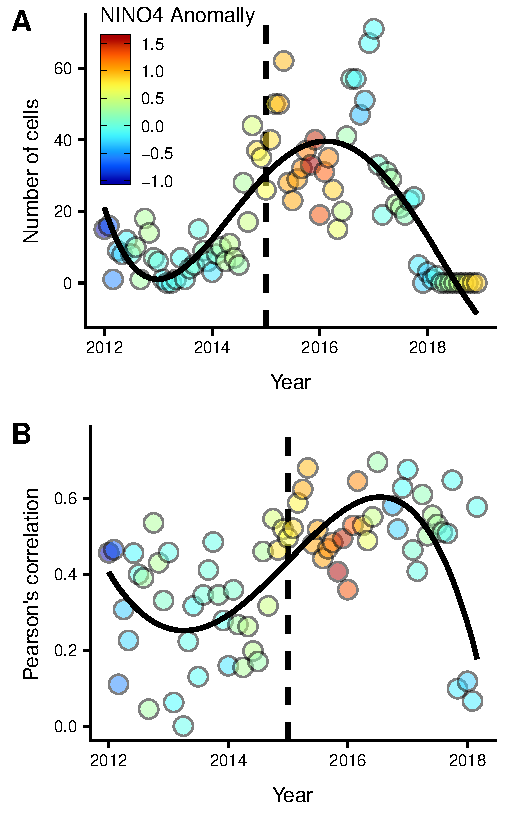
\includegraphics{img/KIR_sp_corr.pdf}
\caption{\label{fig:KIR_sp_corr}Number of cells that had displaced and non-displaced vessels (A) and spatial correlation in the presence-absence of each group per cell (B). The solid lines represent the 4\textsuperscript{th} degree polynomial fit reported in \ref{tab:sp_corr}. Note that the late 2016 and early 2017 showed negative or neutral NINO4 anomalies, similar to those in the pre-PIPA period.}
\end{figure}


\begin{table}[!htbp] \centering 
  \caption{\label{tab:main_DID}Difference-in-differences estimates for our 10 variables of interest: 1) Daily fishing hours, 2) Daily non-fishing at-sea hours, 3) Daily proportion of fishing hours to total at-sea hours, 4) Daily distance traveled, 5) Daily mean distance from port for fishing events, 6) Daily mean distance from shore for fishing events, 7) Monthly fishing hours spent in Kiribati waters, 8) Monthly fishing hours spent in PNA waters. Numbers in parentheses are heteroskedastic-robust standard errors.} 
  \label{} 
\footnotesize 
\begin{tabular}{@{\extracolsep{1pt}}lcccccccc} 
\\[-1.8ex]\hline 
\hline \\[-1.8ex] 
\\[-1.8ex] & (1) & (2) & (3) & (4) & (5) & (6) & (7) & (8)\\ 
\hline \\[-1.8ex] 
 Constant & 0.497$^{***}$ & 3.607$^{***}$ & 0.075$^{***}$ & 5.203$^{***}$ & 12.997$^{***}$ & 12.461$^{***}$ & 3.678$^{***}$ & 4.445$^{***}$ \\ 
  & (0.022) & (0.012) & (0.004) & (0.029) & (0.021) & (0.019) & (0.192) & (0.151) \\ 
  & & & & & & & & \\ 
 Post & 0.839$^{***}$ & $-$0.228$^{***}$ & 0.137$^{***}$ & 0.304$^{***}$ & 0.326$^{***}$ & 0.296$^{***}$ & 1.059$^{***}$ & 1.180$^{***}$ \\ 
  & (0.016) & (0.008) & (0.003) & (0.019) & (0.014) & (0.014) & (0.140) & (0.109) \\ 
  & & & & & & & & \\ 
 Treated & 0.136$^{***}$ & 0.014$^{**}$ & 0.015$^{***}$ & 0.400$^{***}$ & 0.223$^{***}$ & 0.116$^{***}$ & 0.534$^{***}$ & 0.149 \\ 
  & (0.013) & (0.007) & (0.002) & (0.020) & (0.016) & (0.016) & (0.148) & (0.118) \\ 
  & & & & & & & & \\ 
 Post $\times$ Treated & $-$0.244$^{***}$ & 0.013 & $-$0.034$^{***}$ & $-$0.483$^{***}$ & $-$0.281$^{***}$ & $-$0.155$^{***}$ & $-$0.565$^{***}$ & $-$0.399$^{***}$ \\ 
  & (0.019) & (0.009) & (0.003) & (0.022) & (0.017) & (0.017) & (0.161) & (0.127) \\ 
  & & & & & & & & \\ 
\hline \\[-1.8ex] 
Month FE & Yes & Yes & Yes & Yes & Yes & Yes & Yes & Yes \\ 
Flag FE & Yes & Yes & Yes & Yes & Yes & Yes & Yes & Yes \\ 
Observations & 83,052 & 83,052 & 83,051 & 64,387 & 32,055 & 32,055 & 1,814 & 2,588 \\ 
R$^{2}$ & 0.102 & 0.072 & 0.107 & 0.028 & 0.062 & 0.080 & 0.113 & 0.198 \\ 
\hline 
\hline \\[-1.8ex] 
\textit{Note:}  & \multicolumn{8}{r}{$^{*}$p$<$0.1; $^{**}$p$<$0.05; $^{***}$p$<$0.01} \\ 
\end{tabular} 
\end{table} 


\begin{figure}[H]
\centering
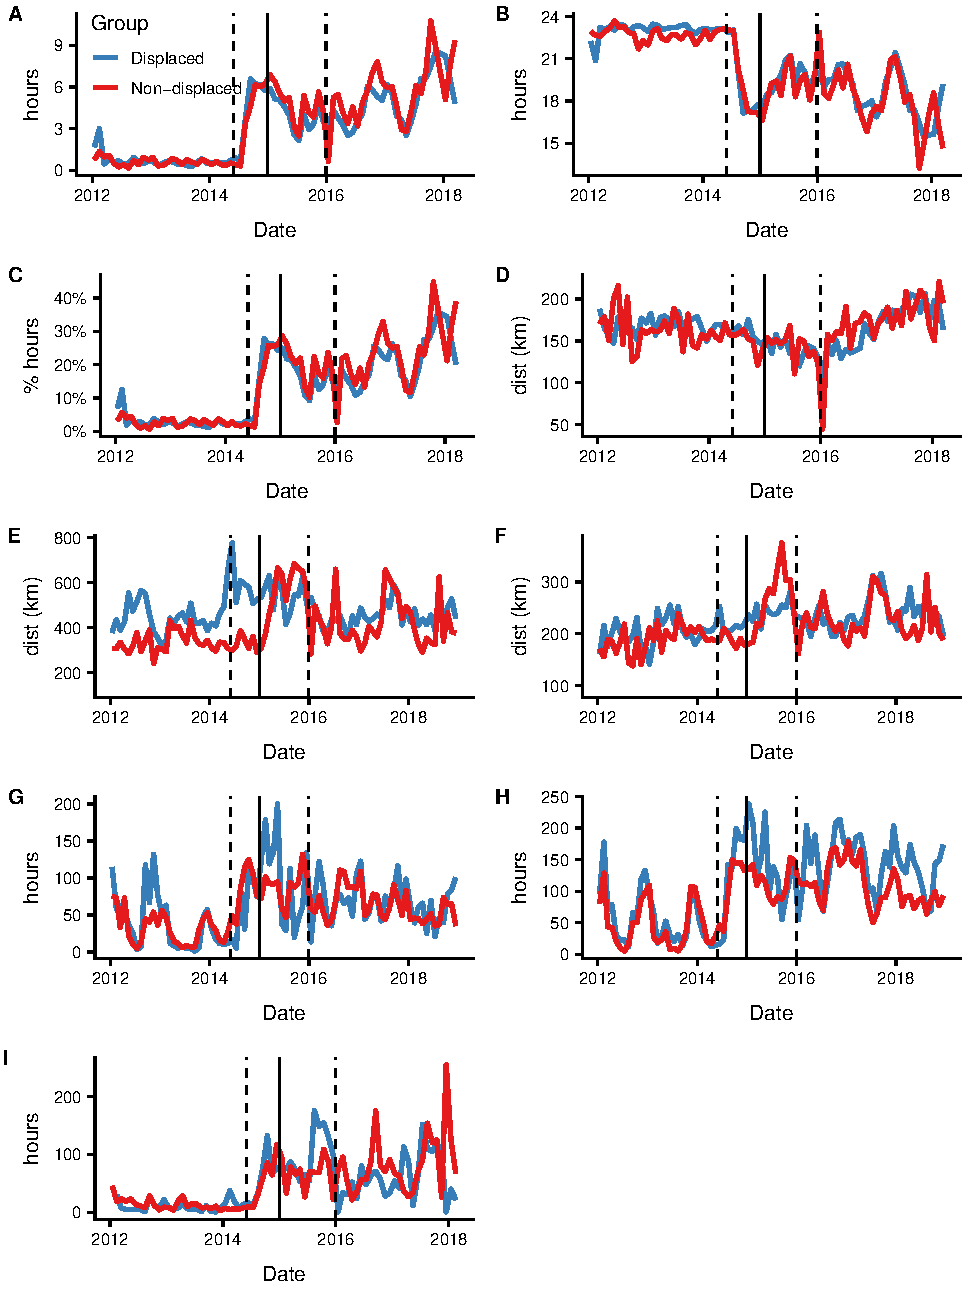
\includegraphics{img/all_panels.pdf}
\caption{\label{fig:all_panels}Time series showing monthly averages for our nine variables of interest: A) Fishing hours, B) Non-fishing hours at-sea, C) Proportion of fishing hours to total hours at-sea, D) Distance traveled, E) Mean distance from port for fishing evetns, F) Mean distance from shore for fishing events, G) Monthly hours spent in Kiribati waters, H) Monthly hours spent in PNA waters, I) Monthly hours spent on the high seas. Dashed vertical lines indicate the addition of new AIS satellites. Solid vertical line indicates the closure of PIPA.}
\end{figure}

\begin{figure}[H]
\centering
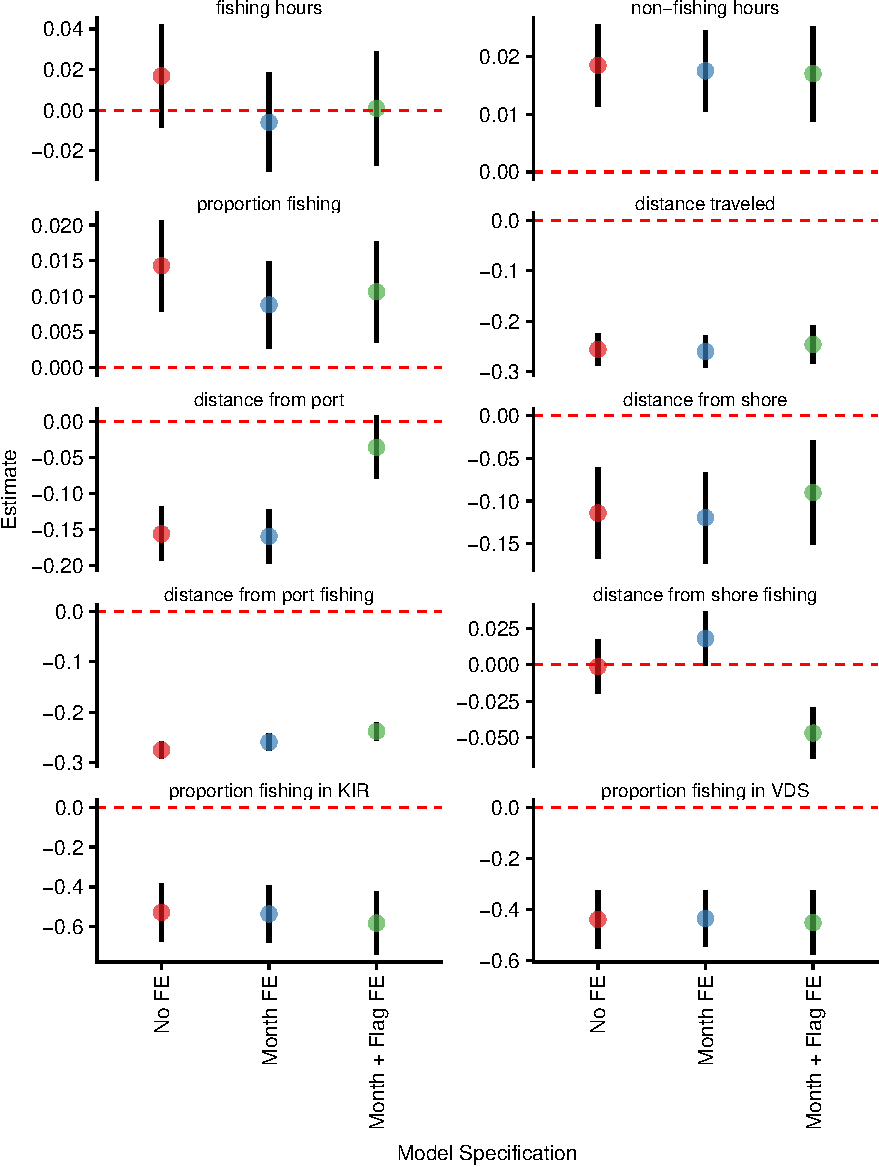
\includegraphics{img/other_specifications.pdf}
\caption{\label{fig:other_specifications}Alternative difference-in-differences estimates for our variables of interest using different model specifications. Table \ref{tab:main_DID} reports estimates for models with month and flag fixed effects, and NINO4 index (\emph{i.e.} green dots).}
\end{figure}


\begin{table}[!htbp] \centering 
  \caption{\label{tab:main_DID}Difference-in-differences estimates for our 10 variables of interest: 1) Daily fishing hours, 2) Daily non-fishing at-sea hours, 3) Daily proportion of fishing hours to total at-sea hours, 4) Daily distance traveled, 5) Daily mean distance from port for fishing events, 6) Daily mean distance from shore for fishing events, 7) Monthly fishing hours spent in Kiribati waters, 8) Monthly fishing hours spent in PNA waters. Numbers in parentheses are heteroskedastic-robust standard errors.} 
  \label{} 
\footnotesize 
\begin{tabular}{@{\extracolsep{1pt}}lcccccccc} 
\\[-1.8ex]\hline 
\hline \\[-1.8ex] 
\\[-1.8ex] & (1) & (2) & (3) & (4) & (5) & (6) & (7) & (8)\\ 
\hline \\[-1.8ex] 
 Constant & 2.449$^{***}$ & 3.325$^{***}$ & 0.314$^{***}$ & 6.177$^{***}$ & 13.800$^{***}$ & 13.159$^{***}$ & 3.979$^{***}$ & 4.644$^{***}$ \\ 
  & (0.061) & (0.031) & (0.014) & (0.042) & (0.047) & (0.065) & (0.392) & (0.343) \\ 
  & & & & & & & & \\ 
 Post & 0.336$^{***}$ & $-$0.353$^{***}$ & 0.083$^{***}$ & 0.105$^{***}$ & 0.398$^{***}$ & 0.352$^{***}$ & 1.151$^{***}$ & 1.240$^{***}$ \\ 
  & (0.024) & (0.015) & (0.006) & (0.020) & (0.016) & (0.016) & (0.157) & (0.125) \\ 
  & & & & & & & & \\ 
 Treated & $-$0.085$^{***}$ & 0.060$^{***}$ & $-$0.028$^{***}$ & 0.259$^{***}$ & 0.259$^{***}$ & 0.163$^{***}$ & 0.435$^{***}$ & 0.082 \\ 
  & (0.027) & (0.014) & (0.007) & (0.020) & (0.018) & (0.018) & (0.163) & (0.133) \\ 
  & & & & & & & & \\ 
 Post $\times$ Treated & 0.036 & $-$0.052$^{***}$ & 0.019$^{***}$ & $-$0.296$^{***}$ & $-$0.342$^{***}$ & $-$0.199$^{***}$ & $-$0.481$^{***}$ & $-$0.335$^{**}$ \\ 
  & (0.028) & (0.017) & (0.007) & (0.024) & (0.020) & (0.019) & (0.179) & (0.142) \\ 
  & & & & & & & & \\ 
\hline \\[-1.8ex] 
Month FE & Yes & Yes & Yes & Yes & Yes & Yes & Yes & Yes \\ 
Flag FE & Yes & Yes & Yes & Yes & Yes & Yes & Yes & Yes \\ 
Observations & 25,004 & 51,724 & 25,004 & 52,767 & 25,004 & 25,004 & 1,399 & 2,010 \\ 
R$^{2}$ & 0.066 & 0.092 & 0.067 & 0.011 & 0.073 & 0.095 & 0.141 & 0.230 \\ 
\hline 
\hline \\[-1.8ex] 
\textit{Note:}  & \multicolumn{8}{r}{$^{*}$p$<$0.1; $^{**}$p$<$0.05; $^{***}$p$<$0.01} \\ 
\end{tabular} 
\end{table} 



\begin{table}[!htbp] \centering 
  \caption{\label{tab:main_DID}Difference-in-differences estimates for our 10 variables of interest: 1) Daily fishing hours, 2) Daily non-fishing at-sea hours, 3) Daily proportion of fishing hours to total at-sea hours, 4) Daily distance traveled, 5) Daily mean distance from port for fishing events, 6) Daily mean distance from shore for fishing events, 7) Monthly fishing hours spent in Kiribati waters, 8) Monthly fishing hours spent in PNA waters. Numbers in parentheses are heteroskedastic-robust standard errors.} 
  \label{} 
\footnotesize 
\begin{tabular}{@{\extracolsep{1pt}}lcccccccc} 
\\[-1.8ex]\hline 
\hline \\[-1.8ex] 
\\[-1.8ex] & (1) & (2) & (3) & (4) & (5) & (6) & (7) & (8)\\ 
\hline \\[-1.8ex] 
 Constant & 2.637$^{***}$ & 3.247$^{***}$ & 0.404$^{***}$ & 5.016$^{***}$ & 13.177$^{***}$ & 12.684$^{***}$ & 3.259$^{***}$ & 4.096$^{***}$ \\ 
  & (0.042) & (0.021) & (0.011) & (0.044) & (0.028) & (0.025) & (0.270) & (0.206) \\ 
  & & & & & & & & \\ 
 Post & 0.283$^{***}$ & $-$0.443$^{***}$ & 0.048$^{***}$ & 0.628$^{***}$ & 0.164$^{***}$ & 0.077$^{***}$ & 1.347$^{***}$ & 1.586$^{***}$ \\ 
  & (0.039) & (0.021) & (0.011) & (0.044) & (0.024) & (0.022) & (0.234) & (0.188) \\ 
  & & & & & & & & \\ 
 Treated & $-$0.091$^{**}$ & $-$0.051$^{***}$ & $-$0.052$^{***}$ & 0.683$^{***}$ & 0.137$^{***}$ & $-$0.020 & 0.697$^{***}$ & 0.477$^{***}$ \\ 
  & (0.040) & (0.019) & (0.011) & (0.041) & (0.024) & (0.022) & (0.233) & (0.184) \\ 
  & & & & & & & & \\ 
 Post $\times$ Treated & 0.081$^{*}$ & 0.021 & 0.055$^{***}$ & $-$0.880$^{***}$ & $-$0.153$^{***}$ & 0.017 & $-$0.691$^{***}$ & $-$0.706$^{***}$ \\ 
  & (0.042) & (0.023) & (0.011) & (0.046) & (0.027) & (0.024) & (0.251) & (0.202) \\ 
  & & & & & & & & \\ 
\hline \\[-1.8ex] 
Month FE & Yes & Yes & Yes & Yes & Yes & Yes & Yes & Yes \\ 
Flag FE & Yes & Yes & Yes & Yes & Yes & Yes & Yes & Yes \\ 
Observations & 19,971 & 42,555 & 19,971 & 43,068 & 19,971 & 19,971 & 1,207 & 1,696 \\ 
R$^{2}$ & 0.064 & 0.097 & 0.066 & 0.032 & 0.059 & 0.071 & 0.133 & 0.217 \\ 
\hline 
\hline \\[-1.8ex] 
\textit{Note:}  & \multicolumn{8}{r}{$^{*}$p$<$0.1; $^{**}$p$<$0.05; $^{***}$p$<$0.01} \\ 
\end{tabular} 
\end{table} 



\begin{table}[H] \centering 
  \caption{\label{tab:DID_without_USA_TWN}Difference-in-differences estimates for our 9 variables of interest after excluding US and Tawianese vessels. 1) Daily fishing hours, 2) Daily non-fishing at-sea hours, 3) Daily proportion of fishing hours to total at-sea hours, 4) Daily distance traveled, 5) Daily mean distance from port for fishing events, 6) Daily mean distance from shore for fishing events, 7) Monthly fishing hours spent in Kiribati waters, 8) Monthly fishing hours spent in PNA waters, and 9) Monthly fishing hours in the high seas. Numbers in parentheses are heteroskedastic-robust standard errors.} 
  \label{} 
\footnotesize 
\begin{tabular}{@{\extracolsep{1pt}}lccccccccc} 
\\[-1.8ex]\hline 
\hline \\[-1.8ex] 
\\[-1.8ex] & (1) & (2) & (3) & (4) & (5) & (6) & (7) & (8) & (9)\\ 
\hline \\[-1.8ex] 
 Constant & 0.536$^{***}$ & 3.600$^{***}$ & 0.082$^{***}$ & 4.506$^{***}$ & 13.002$^{***}$ & 12.438$^{***}$ & 3.850$^{***}$ & 4.719$^{***}$ & 2.420$^{***}$ \\ 
  & (0.023) & (0.012) & (0.004) & (0.043) & (0.022) & (0.020) & (0.209) & (0.158) & (0.419) \\ 
  & & & & & & & & & \\ 
 Post & 0.796$^{***}$ & $-$0.217$^{***}$ & 0.130$^{***}$ & 0.021 & 0.290$^{***}$ & 0.291$^{***}$ & 0.870$^{***}$ & 0.894$^{***}$ & 0.732$^{**}$ \\ 
  & (0.019) & (0.010) & (0.003) & (0.035) & (0.016) & (0.016) & (0.156) & (0.121) & (0.291) \\ 
  & & & & & & & & & \\ 
 Displaced & 0.142$^{***}$ & 0.016$^{**}$ & 0.015$^{***}$ & 0.341$^{***}$ & 0.227$^{***}$ & 0.127$^{***}$ & 0.490$^{***}$ & $-$0.017 & $-$0.296 \\ 
  & (0.013) & (0.007) & (0.002) & (0.031) & (0.018) & (0.017) & (0.163) & (0.126) & (0.239) \\ 
  & & & & & & & & & \\ 
 NINO4 & $-$0.001 & $-$0.001 & 0.001 & $-$0.383$^{***}$ & 0.189$^{***}$ & 0.082$^{***}$ & 0.325$^{***}$ & 0.171$^{***}$ & 0.441$^{***}$ \\ 
  & (0.011) & (0.006) & (0.002) & (0.019) & (0.009) & (0.008) & (0.075) & (0.063) & (0.122) \\ 
  & & & & & & & & & \\ 
 Post $\times$ Displaced & $-$0.212$^{***}$ & $-$0.002 & $-$0.029$^{***}$ & $-$0.158$^{***}$ & $-$0.328$^{***}$ & $-$0.184$^{***}$ & $-$0.533$^{***}$ & $-$0.225 & 0.339 \\ 
  & (0.021) & (0.010) & (0.004) & (0.039) & (0.019) & (0.018) & (0.175) & (0.138) & (0.291) \\ 
  & & & & & & & & & \\ 
\hline \\[-1.8ex] 
Month FE & Yes & Yes & Yes & Yes & Yes & Yes & Yes & Yes & Yes \\ 
Flag FE & Yes & Yes & Yes & Yes & Yes & Yes & Yes & Yes & Yes \\ 
Observations & 73,717 & 73,717 & 73,716 & 73,778 & 26,920 & 26,920 & 1,546 & 2,236 & 660 \\ 
R$^{2}$ & 0.095 & 0.072 & 0.102 & 0.021 & 0.077 & 0.094 & 0.111 & 0.169 & 0.256 \\ 
\hline 
\hline \\[-1.8ex] 
\textit{Note:}  & \multicolumn{9}{r}{$^{*}$p$<$0.1; $^{**}$p$<$0.05; $^{***}$p$<$0.01} \\ 
\end{tabular} 
\end{table} 


\begin{figure}[H]
\centering
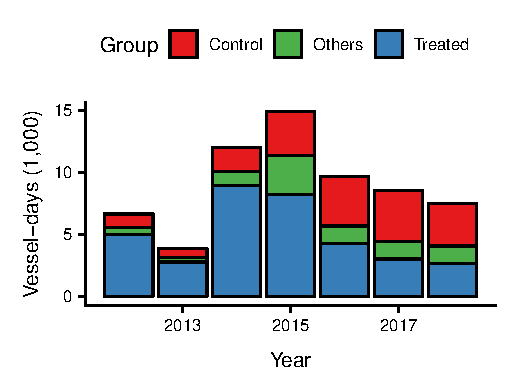
\includegraphics{img/all_PS_VDS_KIR_year.pdf}
\caption{\label{fig:all_PS_VDS_KIR_year}Annual vessel-days in Kiribati by group of vessels.}
\end{figure}

\begin{figure}[H]
\centering
	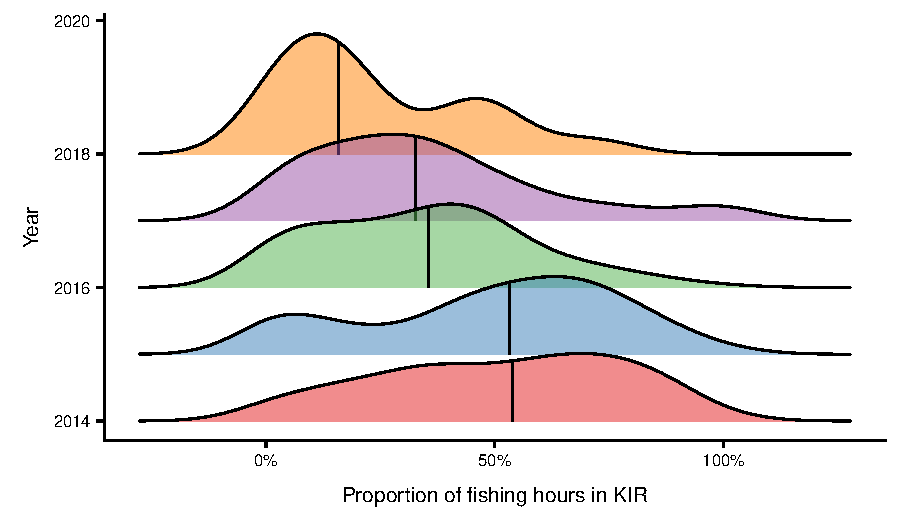
\includegraphics{img/hist_kir_fishing.pdf}
	\caption{\label{fig:hist_kir_fishing}Ridgeplot for the density of the \% of total fishing hours that take place within Kiribati EEZ waters by year for displaced vessels where the unit of observation is an individual vessel.}	
\end{figure}

\begin{figure}[H]
\centering
	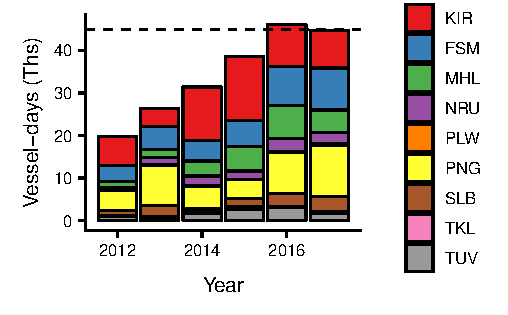
\includegraphics{img/all_PS_VDS_cty_year.pdf}
	\caption{\label{fig:all_PS_VDS_cty_year}Annual vessel-days for all PNA countries, by country.}
\end{figure}

\begin{figure}[H]
\centering
	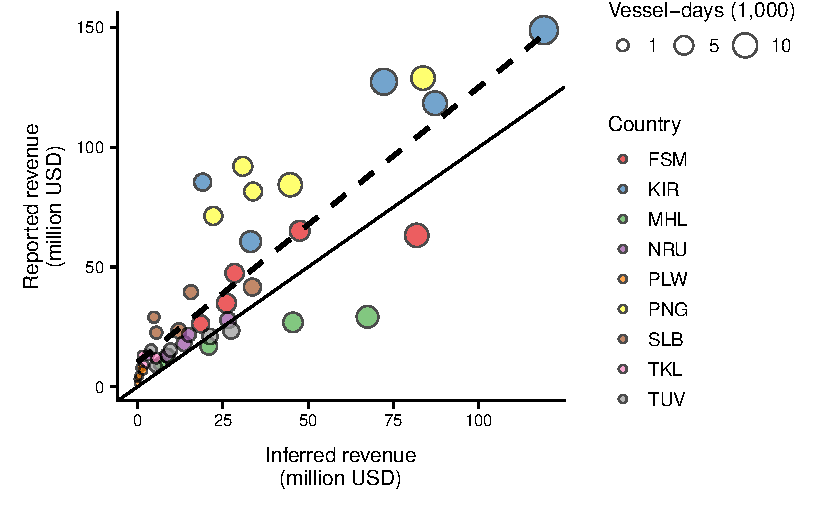
\includegraphics{img/revenue_FFA_GFW_linear.pdf}
	\caption{\label{fig:revenue_FFA_GFW_linear}Inferred revenues vs. reported revenues. The dashed line represents line of best fit, and the solid line represents a 1:1 line.}
\end{figure}

\begin{figure}[H]
\centering
	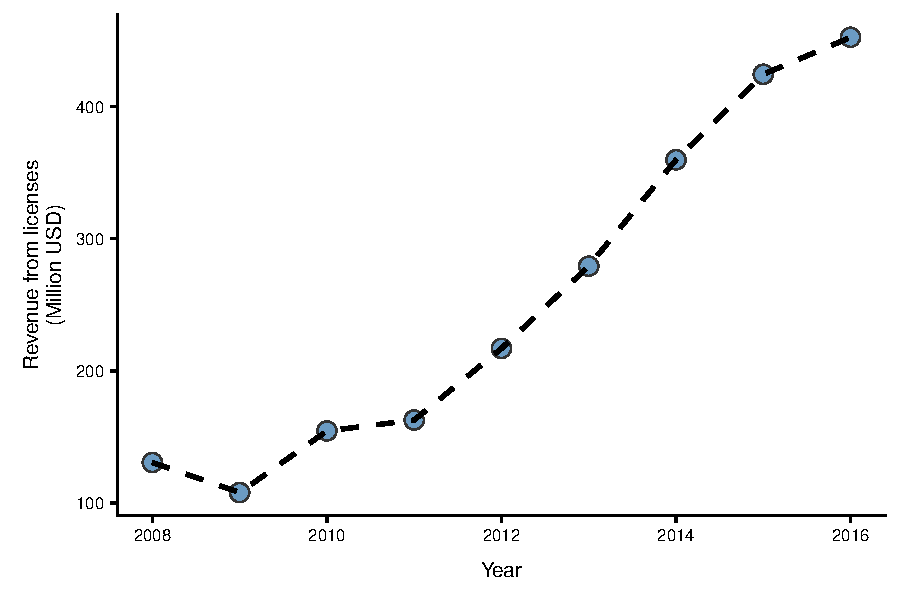
\includegraphics{img/total_PNA_revenues.pdf}
	\caption{\label{fig:total_PNA_revenues}Total revenues for all PNA countries combined.}
\end{figure}

\begin{figure}[H]
\centering
	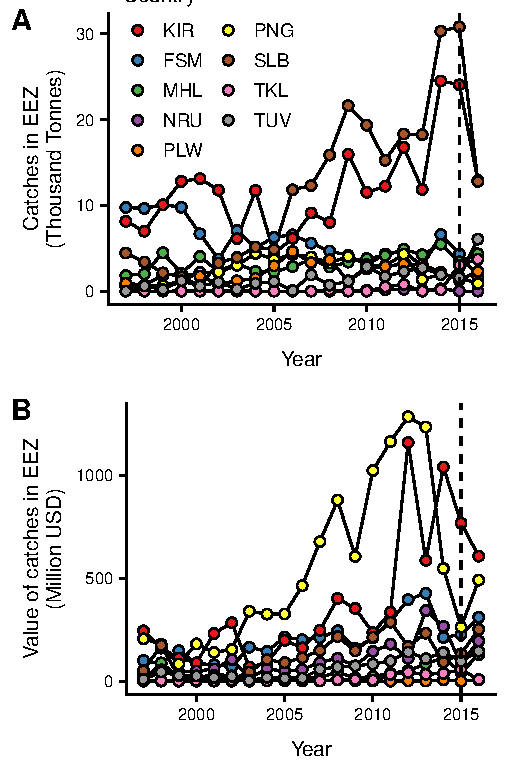
\includegraphics{img/catches.pdf}
	\caption{\label{fig:catches}Financial indicators for PNA countries. A) Annual catches by EEZ and, B) Annual value of catches by EEZ. Vertical dashed line in both plots denotes implementation of PIPA.}
\end{figure}

\begin{figure}[H]
\centering
	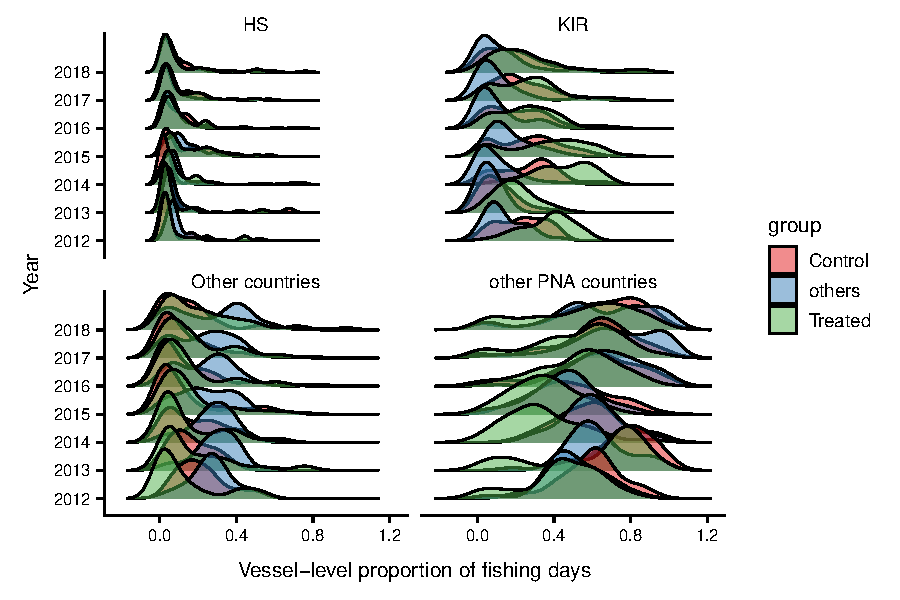
\includegraphics{img/yearly_distribution_prop_fishing_by_region.pdf}
	\caption{\label{fig:yearly_distribution_prop_fishing_by_region}Ridgeplot for the density of the \% of total fishing hours that take place in each region for all vessels}	
\end{figure}

\begin{figure}[H]
\centering
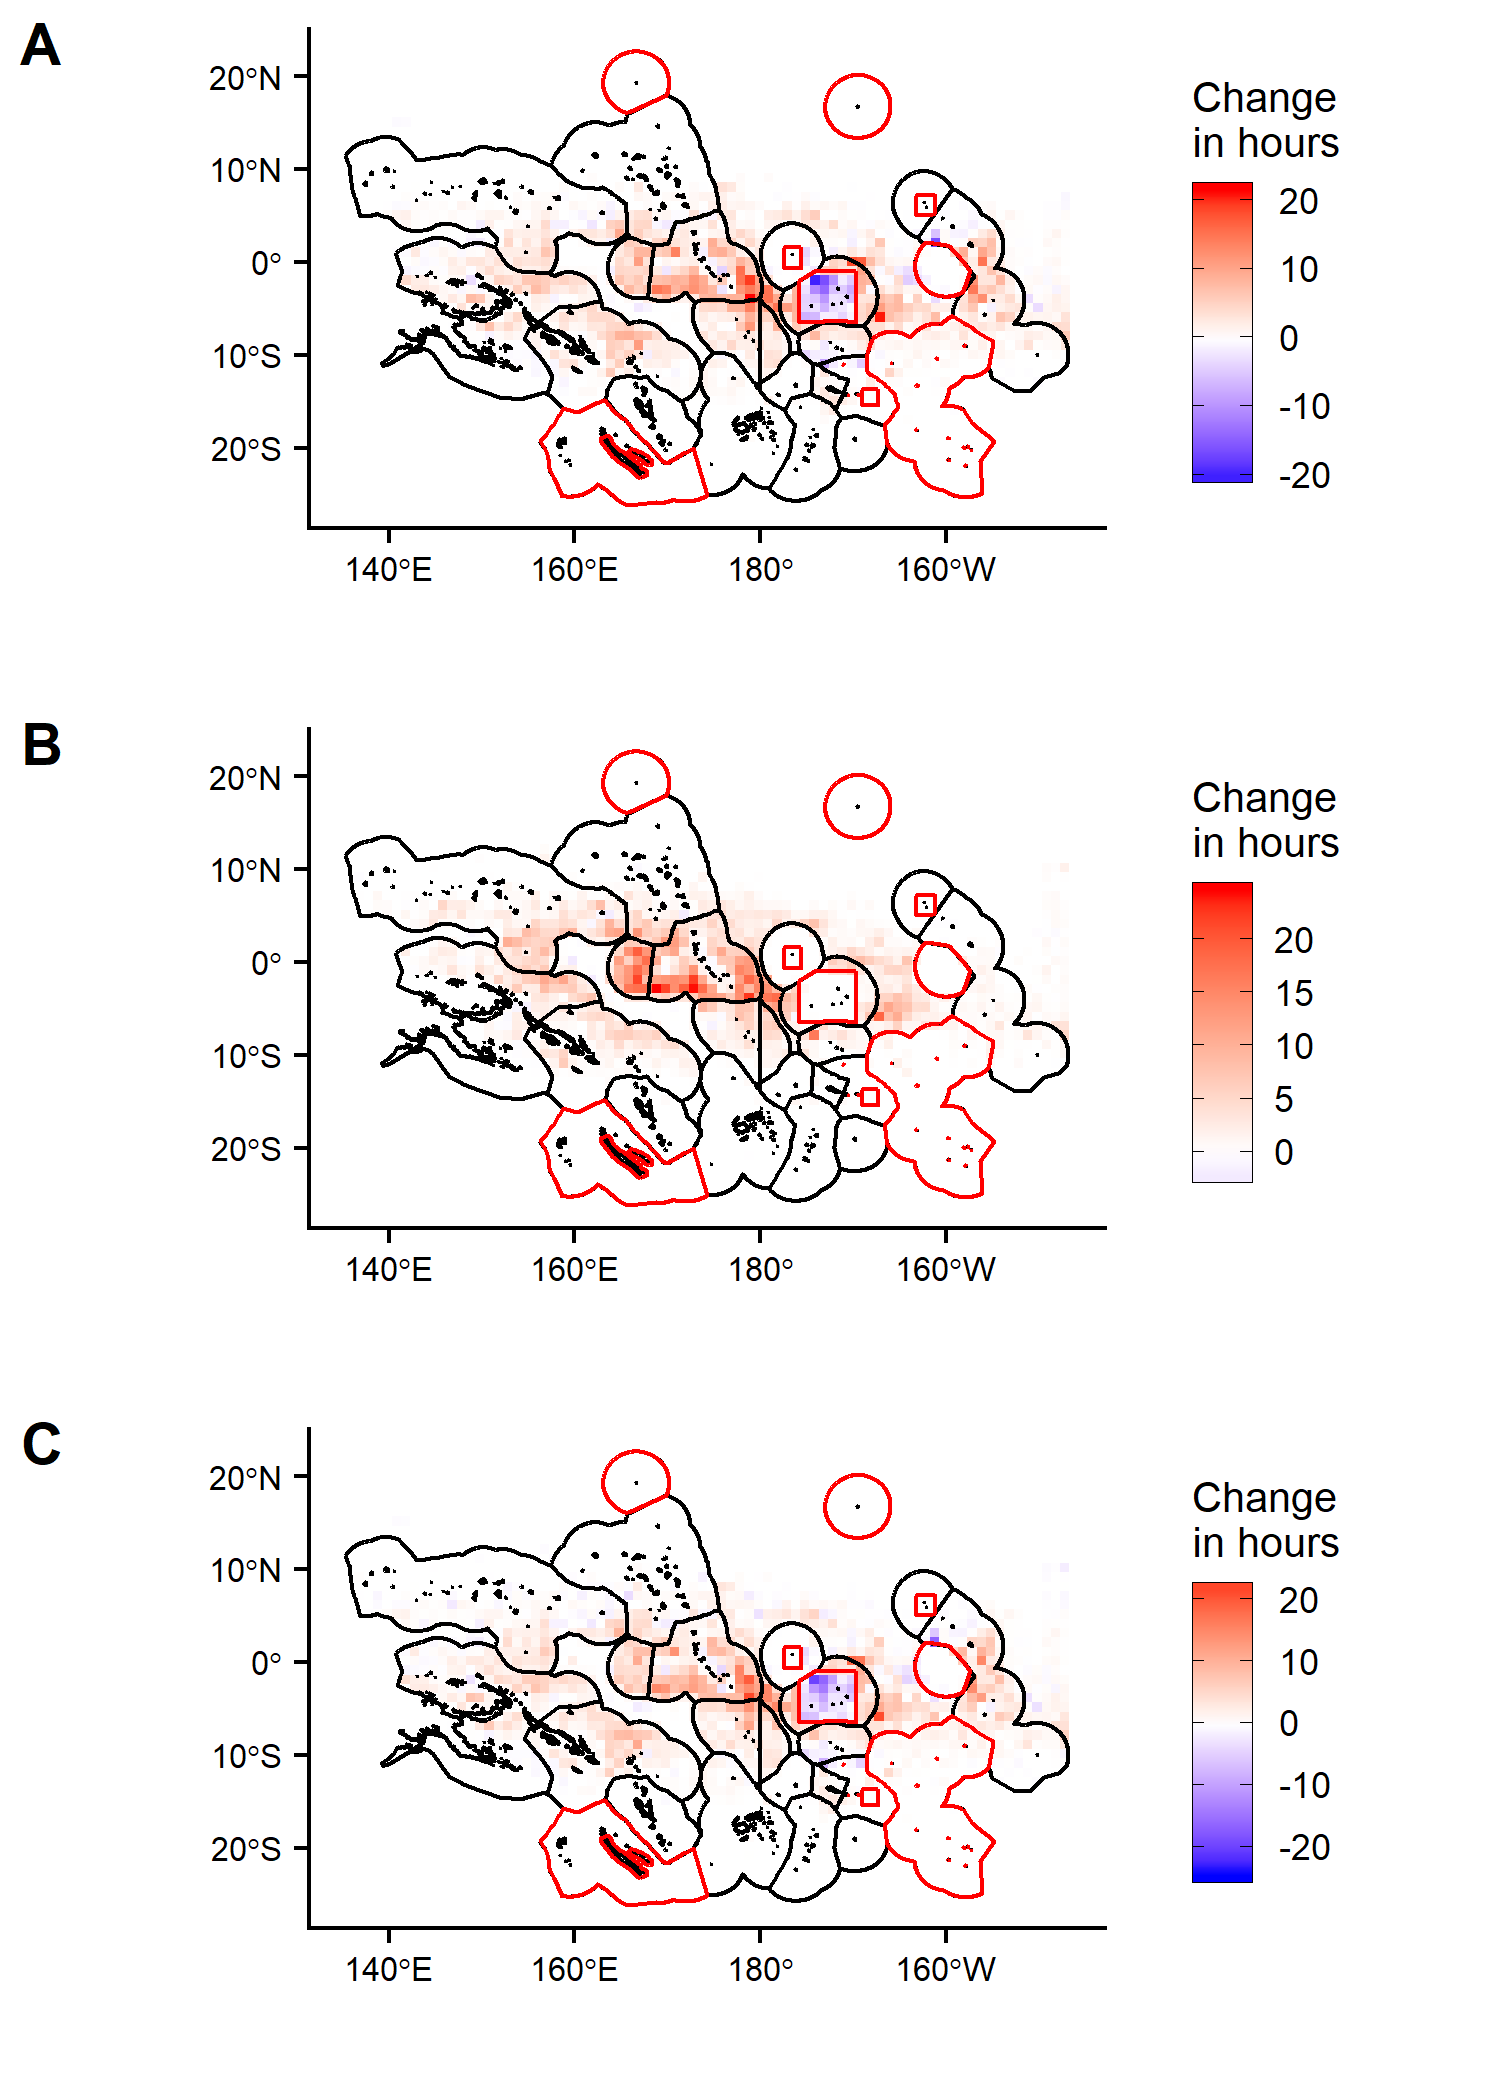
\includegraphics{img/fishing_raster_diff.png}
\caption{\label{fig:fishing_raster_diff}Change in spatial footrpint of analysed vessels. Black lines show Exclusive Economic Zone (EEZ), red lines show existing Marine Protected Areas. Panels A and B show the change through time (after - before) for dislpaced and non-displaced vesels, respectively. Panel C shows the difference between A and B (displaced - non-displaced), highlighting areas where displaced vessels redistributed to, relative to non-displaced vessels. Note that displaced vessels allocate more hours to the Gilbert Islands and Line islands EEZs, but also Tuvalu and the high seas surrounding PIPA.}
\end{figure}

\begin{figure}[H]
\centering
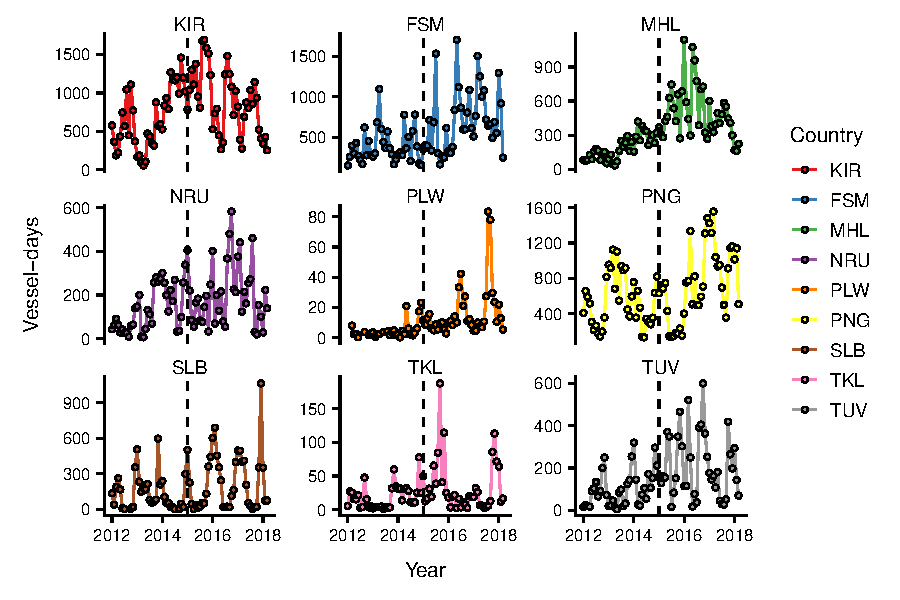
\includegraphics{img/PS_VDS_PNA_by_month_eez.pdf}
\caption{\label{PS_VDS_PNA_by_month_eez}Time series of monthly observed vessel-days for each PNA country.}
\end{figure}

\begin{figure}[H]
\centering
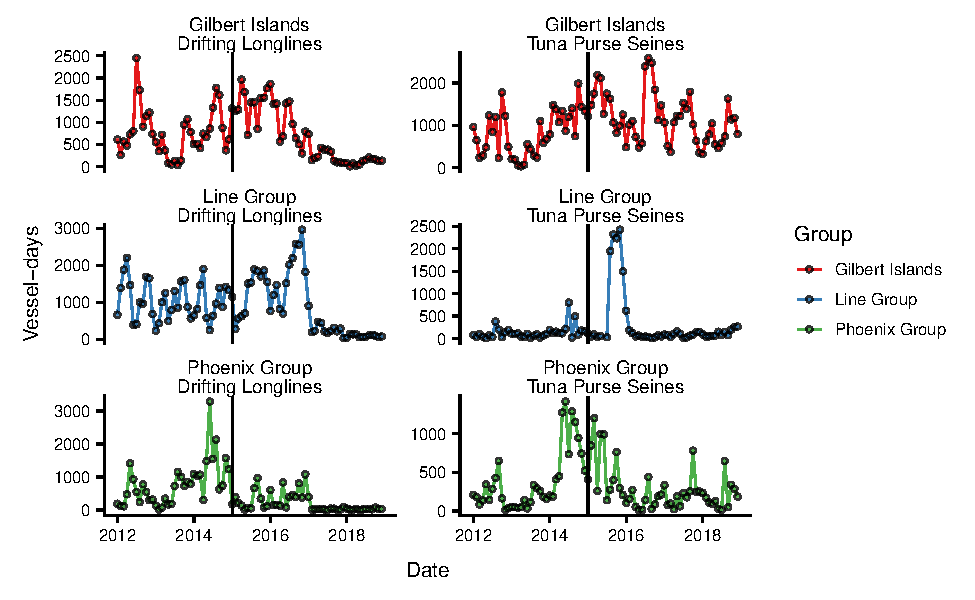
\includegraphics{img/time_series_gear_group.pdf}
\caption{\label{fig:time_series_gear_group}Time series of monthly observed vessel days for drifting longliners and tuna purse seiners in each EEZ belonging to Kiribati: Gilbert islands, Phoenix islands, and Line islands. \emph{I would take this one out, but left it here so you could see the drop in longlines happens later (2017), not aligned with PIPA at all.}}
\end{figure}

\begin{figure}[H]
\centering
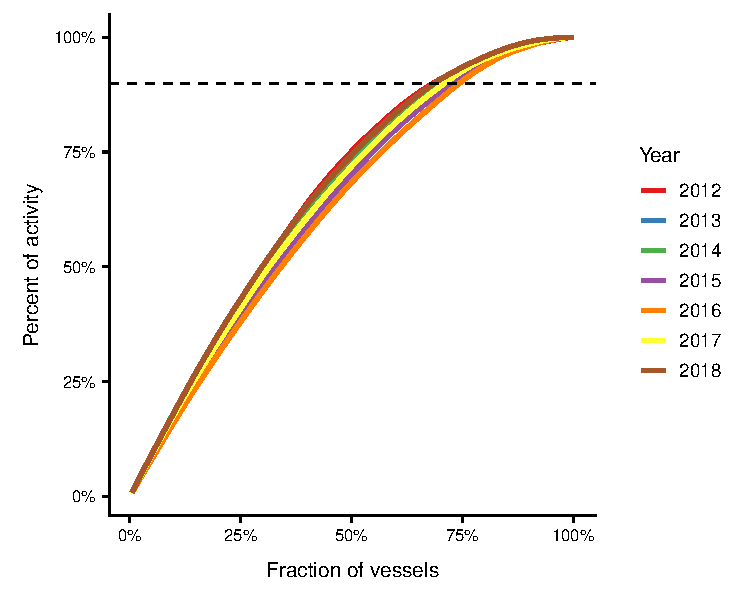
\includegraphics{img/nvessels_to_90.pdf}
\caption{\label{fig:nvessels_to_90}Cumulative activity (\% of total hours) as a function og increasing fraction of vessels (\% of total) by year.)}
\end{figure}



%\section{Old Text}

%\subsection{Large-Scale Marine Protected Areas}\label{lsmpas}
%
%The cutoff at which an MPA is considered to be a LSMPA ranges from areas
%larger than 30,000 km\textsuperscript{2} as defined by
%\cite{desanto_2013} or areas larger than 250,000 km\textsuperscript{2},
%as defined by \cite{toonen_2013}. Figure \ref{fig:LSMPAs_map} shows
%LSMPAs that meet the latter condition, and are also fully no-take. LSMPAs are often
%implemented in the pelagic environment, where the dominant human
%activity is industrial fishing \cite{gray_2017,kroodsma_2018}. The
%early literature on LSMPAs focused on the inherent challenges and
%difficulties that come with a pelagic environment. \cite{kaplan_2010}
%claimed that very large MPAs would result in excessive opportunity costs
%and that these would be difficult to enforce. \cite{game_2009}
%suggested that most of the challenges could be overcome with the
%incorporation of technology, in what then became known as Dynamic Ocean
%Management \citep{maxwell_2015}.\footnote{See \cite{singleton_2014}, who provide an objective discussion of the pros and cons of LSMPAs.} 
%
%Spatial closures of this magnitude are likely to induce changes in
%fishers' behavior. Theoretical models of fishing effort redistribution
%range from the simplistic assumption that effort inside the bounded
%region disappears, to spatially explicit models that reallocate fishing
%effort based on habitat characteristics, presence of other vessels, and
%expected returns \citep{smith_2003,hilborn_2006}. However, these focus
%on the long term optimal equilibrium, and redistribution of fishing
%effort may not always be optimally distributed, especially over the first few years
%\citep{stevenson_2013}.
%
%The empirical research that has been done in smaller sized MPAs
%suggests that resource users may show idiosyncratic responses. For
%example, \cite{stevenson_2013} show that a network of MPAs displaced
%fishing effort farther away from ports, resulting in higher
%\emph{perceived} costs, and increases in catch per unit effort.
%\cite{cabral_2017} analyze the redistribution of fishing and
%non-fishing vessels following the implementation of a network of MPAs in
%California, and find that dive boats follow a
%fishing-the-line pattern, while some fishing boats follow an ideal free
%distribution. More recently \cite{elahi_2018} used satellite tracking
%data to show that a temporal spatial closure caused trawlers to maintain
%effort but apply it more intensively elsewhere, particularly along the
%borders and closer to shore. The way in which fishers react to a spatial
%closure can have major implications for its outcome
%\citep{smith_2003,hilborn_2006}, highlighting the need to understand how
%fishers react to the implementation of LSMPAs, how fishing effort
%changes, and how it is spatially redistributed. All these studies evaluate relatively small closures within Exclusive Economic Zones, where other regulations exist.
%This may not always be the case for LSMPAs, where often the entire EEZ
%is converted into a LSMPA, leaving fishers with the option of moving to
%the high seas or other countries' EEZs, with potentially very different fishing regulations.
%
%\subsection{Nauru agreement and the Phoenix Islands Protected Area}
%
%The cooperation that emerged under the Nauru Agreement allowed for subsequent
%agreements that strengthened fisheries management, like the Palau
%Agreement, which limited the number of purse seiners at 205 vessels from
%1995-2007.\footnote{See \cite{havice_2010} for a detailed description of the Nauru, Palau, and Federated States of Micronesia agreements.} However, the most notable regulation is
%the approach to manage fishing effort: a Vessel Day Scheme (VDS)
%implemented in 2007 \citep{havice_2013}. This effectively modified how
%fishing effort was managed, from total number of vessels (under the Palau
%Agreement) to total vessel-days. 
%Under the purse seine VDS, a total number of annual vessel days for the entire fishery is agreed upon by the PNA parties. Each party’s allowable effort (PAE) is then calculated based on historic effort and biomass within each party’s EEZ. Sixty percent of the PAE is calculated based on EEZ effort over the last seven years and 40\% of the PAE is calculated based on the 10-year average of each country’s share of estimated skipjack and yellowfin biomass within its EEZ.\footnote{This is explained in more detail in Article 12.5 of the 2012 Amendment to the Palau Agreement and in \cite{Hagrannsoknir2014}}. A minimum benchmark fee is set for purse seine vessel days which each party can transfer (\emph{i.e.} sell to another PNA member) or sell to the highest bidder (\emph{i.e.} sell to a fishing company). Vessel days can be transferred to fish in any PNA party’s EEZ, without penalty to the transferred parties' allocations \cite{PNA2016}.\footnote{The process of transferring days between parties is described in Article 7 of the Management Scheme \cite{PNA2016}.} The mean value of a vessel day has steadily increased since 2007 \citep{havice_2013}. 
%Although detailed records on sales or transfers of vessel days are not publicly available \citep{havice_2013,yeeting2018stabilising}, a minimum benchmark fee of \$8,000/day was set from 2015 \citep{PNA2014a}.
%
%\cite{yeeting2018stabilising} summarize the PNA implementing arrangements as follows: “foreign vessels [are required] to be registered and licensed, report catches, maintain log books, allow observers on board and maintain transparency over their fishing activities.” Further, vessels registered with the Vessel Day Scheme are required to have Automatic Location Communicators (ALC) or Mobile Transceiver Units (MTU) that transmit their locations at least once per hour while they are within the VDS Management Area \citep{PNA2016}. Every entire day that a vessel is within the VDS Management Area is counted as a vessel day used, unless the vessel reports a “no fishing day” (e.g., travel, maintenance, etc.) and periods of less than 24 hours are counted as partial days \citep{PNA2016}.  As described in the Palau Arrangement, fishing days by vessels shorter than 50m (longer than 80m) count as 0.5 (1.5) vessel days. Countries are responsible for ensuring registered vessels comply with the implementing arrangements and that they stay within their PAE. Parties that exceed their PAE should reportedly be penalized by reductions to the following year’s PAE \citep{PNA2016}. There are some criticisms of the PNA PS VDS claiming that there is a lack of monitoring, compliance, and transparency that could hinder the future success of the program \citep{Arnason2014,yeeting2018stabilising}. While the effectiveness of this scheme has been
%debated in terms of meeting fishery management and conservation
%objectives, the licensing significantly contributes to the economy of
%these island nations \citep{havice_2010}.
%
%The main tuna species caught in the region are skipjack
%(\emph{Katsuwonus pelamis}), yellowfin (\emph{Thunnus albacares}),
%albacore (\emph{Thunnus alalunga}) and bigeye (\emph{Thunnus obesus}).
%From these, the first two are amongst the top-10 species represented in
%global fisheries production statistics, with 2016 catches increasing
%relative to the 2005-2014 average \citep{fao_2018}. This region of the
%Pacific has historically accounted for a large portion of tuna catches
%\cite{aqorau_1997}. Today, the PNA controls close to 50\% of global
%skipjack tuna production \cite{pna_website_2018} and the combined area of all EEZs involved is 14.6 million km\textsuperscript{2}, larger than the land mass of the United States of America. A large portion of global skipjack
%catch derives from purse seine vessels licensed under the VDS.
%Fishing vessels from Australia, New Zealand, China, France, Korea,
%Japan, the Philippines, Taiwan, and the United States participate in the
%purse-seining VDS.
%
%One of the most notable and recent management interventions in the
%region is the implementation of the Phoenix Islands Protected Area (PIPA)
%by the government of Kiribati. PIPA was first declared in 2006, and
%established in 2008 with only 4\% of the area declared as no-take. On
%January 1\textsuperscript{st}, 2015, the no-take area within PIPA was
%expanded to a total area of 397,447 km\textsuperscript{2}, roughly 1.5
%times the size of Ecuador. Figure \ref{fig:PNA_map} shows a map of the
%PNA countries (excluding Palau) and the Phoenix Islands Protected Area.
%
%The closure of such a large area in one of the most important fishing
%regions in the world provides a unique opportunity to evaluate the
%behavioral responses and redistribution of fishing effort by vessels
%that used to fish there. PIPA has been the focus of previous research
%showing that fishing effort is effectively reduced after implementation
%\citep{mccauley_2016,mcdermott_2018}. To this, we pose two questions:
%How did individual vessels respond to the sudden exclusion of such a big
%area? Where did all the vessels go? And what does this imply for revenues from
%selling VDS for both Kiribati and the PNA as a whole? 
%
%A spatial closure might cause fishers to modify
%their behavior as they adapt to a new state of the world. For example, some may have
%to travel further distances to find new fishing grounds, increasing their fuel
%costs. If fishers had developed experience for fishing in particular
%sites, being excluded might impose a learning cost on them, as they
%identify new fishing grounds. This might result in increased search
%times. However, if the area of knowledge of a vessel is significantly
%larger than that of the spatial closure, they might already know other
%places to fish. In the next sections we describe
%the data and methods used to answer these questions.
%
%\subsection{Palau}
%
%\subsubsection{Palau National Monument}

%On October 28, 2015, the President of Palau, H.E. Tommy E. Remengesau Jr., signed into law the Palau National Marine Sanctuary (PNMS) Act. Starting in December 2020, this Act will close 500,000 km\textsuperscript{2} to commercial fishing activities, creating the 14th largest protected area in the world. The sanctuary will fully protect about 80 percent of the nation’s EEZ. The remaining 20\% of Palau’s EEZ (close to the most heavily populated islands: Koror and Babeldaob) will become a Domestic Fishing Zone in which traditional and domestic fishing activities will be allowed to provide fish solely for the domestic market (\emph{i.e.} exports of pelagic fish will be prohibited). Alongside these protections, the Palau National Marine Sanctuary (PNMS) Act will support a domestic pelagic fishery. In this section, we use our preceding analysis on the ex-post impacts of PIPA to attempt to make some \emph{ex ante} predictions about the potential impacts of PNMS. We start by giving some background on the fishing that is currently taking place inside the future PNMS. 

%\subsubsection{Background on Commercial Fishing in Palau}

%Foreign tuna fishing in Palau’s EEZ began before WWI. Pole and line was the initial gear used to target skipjack tuna by Japanese vessels. Foreign fishing activities stopped during WWII and started again in the 1960s when Japanese fishers returned and the locally based Van Camp Seafood Company carried out fishing with boats crewed by Okinawans. The Japanese also began purse seine fishing in the 1960s and 1970s and limited longline fishing for yellowfin tuna developed during the same time. During the 1980s, longline fishers began to set their lines deeper, shifting their targets to bigeye tuna. During the 1980s, Korean and Taiwanese vessels also began longline fishing in Palauan waters for export to Japan \citep{chapman2000development}. There are currently three transshipment companies operating in Palau.

%Purse seine vessels target schools of skipjack tuna that are then canned. Compared to other EEZs in the Pacific, especially the PNA EEZs, Palau’s EEZ is not known to be a preferred fishing ground for purse seining (Sisior, pers. comm.). This can be seen in Figure \ref{fig:VDS_country_year}. Currently all purse seine boats fishing in Palau’s EEZ are Japanese and they do not land their catch in Palau (Table \ref{tab:palau_purse}). 



%All longline vessels fishing in Palau’s EEZ are foreign owned (Table \ref{tab:palau_long}). Japanese longline vessels do not land their catch in Palau. Locally-based, foreign-owned longline boats are mostly Taiwanese vessels that are contracted by one of the two main fishing companies (Palau International Traders Incorporated (PITI) and Kuniyoshi Fishing Company (KFC)). Ninety-five percent of the catch from PITI and KFC contracted boats is exported to Japan upon landing in Koror (the largest town in and former capital of Palau). Most of the discards are either sold or donated in Palau. A very small portion of the discards is frozen and transported to Taiwan when vessels return to their home ports.



%\subsubsection{Access fees and taxes}
%
%An agreement between Palau and four Japanese fishing associations\footnote{This is a single agreement between Palau and four associations—1)Federation of Japan Tuna Fisheries Cooperative Associations, 2) National Offshore Tuna Fisheries Association of Japan, 3) Japan Far Seas Purse Seine Fishing Association, 4) Federation of North Pacific District Purse Seine Fisheries Cooperative Association of Japan (Performance Audit Report on Managing Sustainable Fisheries (Tuna) 2013).} covered three methods of fishing (longline, purse seine, and pole and line) and allowed Japan to have up to 290 vessels in Palau waters with no limits on catch. Japan paid 4-5\% of catch returns for this access, but there was no way to validate their catch \citep{Tewid2013}. Between 2010 and 2014, Japan paid Palau between \$196,100- \$867,120 annually in access fees \citep{Gillett2016}. Currently, these access fees have been replaced by the PNA vessel day scheme (described earlier).
% 
%There used to be a number of agreements between the Republic of Palau and foreign owned, local based companies, in particular PITI and KFC, to allow longline fishing \cite{Tewid2013}. Vessels under these agreements were internationally-owned, locally-based vessels that paid for annual licenses based on the size of each vessel. These are the vessels shown in Table \ref{tab:palau_long} (excluding the Japanese vessels). So, for example, there were 38 vessels as part of these agreements in 2016. Between 2010 and 2014, licensing fee revenue from these agreements was between \$219,000-\$284,600 per year \citep{Gillett2016}. These access fees have also been replaced by a new longline-specific version of the VDS (described in more detail below).
%
%There are two multilateral treaties that grant preferential access to Palau waters to US and Federated States of Micronesia (FSM) flagged purse seine boats: the US Multilateral Tuna Treaty and the Federated States of Micronesia Arrangement.  The US Treaty was renegotiated in 2016 with stipulations on minimum vessel day fees. Very little purse seine fishing is conducted by FSM and US vessels in Palau’s EEZ, but Palau still receives a portion of these treaty funds. These agreements have been described by some commentators as foreign aid, with little connection to underlying fish stocks \cite{Gillett2016}. 
%
%The export tax for all commercial tuna and billfish, either fresh or frozen, is \$0.35/kg. Average annual revenue from export taxes was around \$500,000 from 2011-2014 \citep{Gillett2016}. 
%Other than the access fees and tax revenue, Palau receives little additional economic benefits from pelagic fisheries, especially considering that very few jobs are created by the fishery. Between 80 to 90 people are employed by offshore fisheries, and of these only around 20\% are Palauans, earning wages that are only 50\% of average wages in Palau \cite{Gillett2016}.
%
%\subsubsection{Parties to the Nauru Agreement and the Vessel Day Scheme}
%
%In the case of Palau, the VDS is run by the Bureau of Marine Resources, within the Ministry of Natural Resources, Environment and Tourism. Palau’s current purse seine VDS allotment is reportedly around 700 vessel days annually (Sisior, pers. comm., \cite{Pojas2018}), although historically this number has been lower (average of 580 days between 2008-2011 \citep{Tewid2013}). Palau sells most of its vessel days to the US for \$12,500 per day (as negotiated in the US treaty), regardless of whether US vessels actually fish in Palau’s EEZ. The remainder of Palau’s purse seine vessel days are sold for between \$9-10,000 each. When vessel days are purchased to transfer to another EEZ, Palau charges a transfer fee (approximately \$500), for administration costs and future opportunity costs (since vessel day allotments are based partly on historical effort within the EEZ). Though records are confidential, it has been publicly reported that one PNA member party that Palau has transferred vessel days to is Papua New Guinea \citep{Tewid2013} and in 2018, vessel days were sold to a fishing company in the Philippines for the first time \citep{Pojas2018}. In 2018, Palau brought in approximately \$9 million USD in VDS revenue (Sisior pers. comm.). 
%
%The longline VDS (LL VDS) is in its infancy and has not yet been fully implemented at the PNA-scale, although several countries are now implementing it at the country-scale. Palau was the first party to implement the VDS for longline fishing in 2017. In 2014, longline boats fishing in Palau’s EEZ fished 10,500 days (Sisior, pers. comm.). Since 2016, the number of allowed longline VDs has been a fraction of the 2014 days, reducing each year as stipulated in the PNMS Act. Palau sells its LL VD for \$150-\$250 (Sisior pers. comm.). Because the LL VDS is still new and has yet to be fully implemented by all parties, LL VD are not currently transferable between PNA member EEZs. 
%
%\subsubsection{Plans for a domestic pelagic fishery}
%
%In the recent past, a single domestic pole and line vessel supplied Palau with an estimated 100mt of catch \cite{Gillett2016}. The vessel ceased operations in recent years when the captain became ill and passed away, but there is talk that it is gearing up to start operations again under new leadership (Sisior, pers. comm.). Otherwise, there are no domestic vessels dedicated to full-time offshore fishing. A number of fishers occasionally troll offshore for tuna and other pelagics, but there are no official estimates of volumes. 
%Local NGOs have sponsored short trainings on small-scale canning and proper techniques for processing high grade tuna to encourage existing fishers to devote more time to offshore fishing. There are several possible scenarios for a domestic fishery (including those featured in a feasibility report by FFA \citep{Skirtun2017}), but there has yet to be any official action towards a particular scenario.

\end{document}
